\chapter{Evaluación}\label{chapter:evaluation}

Este capítulo describe el diseño experimental y los resultados de la evaluación del sistema propuesto, centrada en la validación empírica de cuatro hipótesis relacionadas con la efectividad de distintas técnicas aplicadas al modelado automático de problemas de planificación. Cada hipótesis busca demostrar la contribución individual de uno o varios componentes específicos al desempeño global del agente modelador basado en \textit{LLMs}, ya sea en términos de correctitud sintáctica, solubilidad o fidelidad semántica del modelo generado:

\begin{itemize}
    \item[\textbf{H1.}] La división del proceso de modelado en fases estructuradas —extracción de objetos, razonamiento, especificación del estado inicial y metas, y generación del archivo \textit{PDDL}— mejora la correctitud de los modelos generados, al permitir un razonamiento más controlado, modular y verificable.
    \item[\textbf{H2.}] La aplicación de \textit{GCD}  permite una generación más confiable del código \textit{PDDL}, reduciendo significativamente o eliminando por completo la aparición de errores de sintaxis.
    \item[\textbf{H3.}] La introducción de reflexión sobre errores y una mínima retroalimentación humana o automática permite al agente corregir patrones de falla recurrentes, contribuyendo al aumento de la solubilidad y la correctitud del \textit{PDDL} generado.
    \item[\textbf{H4.}] La incorporación de \textit{RAG} para la selección de ejemplos relevantes y la extracción de \textit{insights} a partir de soluciones previas (tanto correctas como erróneas), representa una vía prometedora para mejorar la capacidad de los agentes basados en \textit{LLMs} para modelar tareas de planificación, al permitirles adaptarse a la semántica de nuevas tareas y fortalecer su conocimiento sobre el dominio específico y la modelación de problemas.
\end{itemize}

La evaluación se desarrolla en dos fases principales. La primera corresponde a una evaluación comparativa estática, sobre un subconjunto común del \textit{benchmark Planetarium}, en la cual se analiza el comportamiento de múltiples variantes del agente modelador. En esta fase se incluyen, en primer lugar, los agentes planificadores básicos originales introducidos por \textit{LLM+P}, a saber, \textit{LLM-as-P\textsuperscript{-}} (modelo \textit{Zero-Shot}) y \textit{LLM-as-P\textsuperscript{+}} (modelo \textit{One-Shot} con un ejemplo fijo), que no generan código \textit{PDDL} sino directamente planes a partir de descripciones en lenguaje natural. Estos agentes actúan como \textit{baselines} para evaluar la dificultad del \textit{benchmark} y las ventajas del modelado explícito. En segundo lugar, se evalúan también los agentes modeladores de planificación originales de \textit{LLM+P}, esto es, \textit{LLM+P\textsuperscript{-}} y \textit{LLM+P\textsuperscript{+}}, que sí generan archivos de problema en \textit{PDDL} y constituyen un punto de partida relevante para contrastar la efectividad de los módulos propuestos en esta tesis. Los agentes modeladores originales de \textit{LLM+P} se reimplementan para mejorar su \textit{prompt}, adaptarlo mejor a la evaluación en \textit{Planetarium}, y estructurarlo, para que sirva como \textit{baseline} y como el estándar o base sobre la cual se añaden las mejoras propuestas.

A continuación, se consideran variantes del agente propuesto en esta investigación, construidas de manera incremental mediante la incorporación progresiva de módulos diseñados para mejorar la generación de modelos. Estas variantes permiten analizar empíricamente la influencia directa de cada técnica propuesta. Se parte de una reimplementación básica del agente de \textit{LLM+P}, sobre la cual se introducen primero mecanismos de razonamiento estructurado y extracción de objetos —ambos dirigidos a modular el proceso de modelado, conforme a la hipótesis \textbf{H1}—. Luego se incorpora \textit{Grammar-Constrained Decoding (GCD)} para garantizar la validez sintáctica de las salidas, con énfasis especial en su variante condicionada por conocimiento del dominio (\textit{DAPS GCD}), en línea con la hipótesis \textbf{H2}. Además, se aplica \textit{Few-Shot Prompting}, con un ejemplo fijo por dominio, construido manualmente. Todas estas variantes son evaluadas con un \textit{LLM} de gran tamaño y alta capacidad: \textit{Llama 4 Maverick Instruct (Basic)} \parencite{fireworks2025llama4maverick}. 

Complementando esta evaluación comparativa, la segunda fase del experimento aborda el proceso de entrenamiento del agente experiencial, es decir, aquel capaz de realizar reintentos informados y con reflexión autocrítica, y aprovechar información derivada de su experiencia acumulada durante el proceso de entrenamiento previo. Esta fase incluye la acumulación de experiencias exitosas y fallidas (\textbf{H4}), con capacidad de reintentos guiados por \textit{feedback} y autorreflexión (\textbf{H3}), y la extracción automática de \textit{insights} mediante un proceso iterativo controlado por un \textit{LLM} especializado (\textbf{H4}). Esta dinámica se orienta no solo a mejorar el rendimiento del agente en tareas futuras, sino también a evaluar la calidad y utilidad de los conocimientos derivados de la experiencia.

Finalmente, se propone la evaluación sobre el mismo conjunto de evaluación anterior, los agentes modeladores experienciales. Estos agentes integran mecanismos de retroalimentación automática, y reflexión autocrítica sobre errores pasados, asistidos por \textit{LLMs}, o una forma mínima de retroalimentación humana, en el marco de la hipótesis \textbf{H3}. Se realiza la evaluación de los mecanismos de reintento guiado sobre los problemas modelados incorrectamente en los intentos únicos del mejor agente de la fase anterior.

Se exploran también los mecanismos de \textit{FSP} potenciados con \textit{RAG} para seleccionar ejemplos semánticamente similares del \textit{corpus} de soluciones válidas, como se sugiere en \textbf{H4}. En relación con esta misma hipótesis, se prueba la integración de un conjunto de \textit{insights} previamente extraídos del historial de errores y aciertos.

La estructura de este capítulo refleja esta metodología. Primero se describe en detalle el diseño de los experimentos, estableciendo la relación de cada fase con las hipótesis planteadas. Luego se presentan los resultados obtenidos, acompañados de métricas cuantitativas y visualizaciones comparativas. A continuación, se discute críticamente la influencia de cada componente en los resultados, y se identifican observaciones relevantes sobre las interacciones entre técnicas. Finalmente, se exponen las limitaciones de la evaluación, se resumen los resultados obtenidos y se analiza el grado de cumplimiento de cada hipótesis dentro del marco experimental planteado.

\section{Selección de subconjuntos de \textit{Planetarium}}

Para garantizar evaluaciones rigurosas y comparables, el proceso de selección de datos se organizó en tres fases complementarias: muestreo de pares \texttt{(init, goal)}, filtrado estratificado sobre la base SQLite, y generación de subconjuntos finales de evaluación y entrenamiento.

En la primera fase, se definió estáticamente un conjunto amplio de todas las parejas posibles de configuraciones o subtipos de tareas de los estados inicial (\texttt{init}) y objetivo (\texttt{goal}) para cada dominio (\textit{Blocksworld}, \textit{Gripper} y \textit{Floor-Tile}). A partir de estas parejas, se seleccionaron aleatoriamente subconjuntos de casos de entrenamiento y prueba, empleando una semilla fija para asegurar reproducibilidad. Este muestreo inicial permite controlar la cobertura de distintos tipos de tareas.

En la segunda fase, cada pareja elegida se usó para filtrar directamente la tabla \texttt{problems} de la base SQLite, construyendo máscaras que combinan rangos de número de objetos, cantidad de proposiciones en \texttt{:init} y \texttt{:goal}, y niveles de abstracción de los estados (abstracto o explícito). Para cada celda de esta cuadrícula multivariada, se extrajeron hasta \(N\) ejemplos al azar, posibilitando un muestreo estratificado sobre toda la diversidad del dataset.

La tercera fase concluyó la construcción de los subconjuntos:  
\begin{itemize}  
  \item Con los casos de prueba iniciales filtrados, se depuraron duplicados y se agruparon por dominio. Se extrajeron finalmente 16 instancias de \textit{Blocksworld}\footnote{Se obtuvieron menos instancias en este dominio que en el resto debido a que el \textit{split} de evaluación (\textit{test}) de \textit{Planetarium} solo contiene dos parejas de configuraciones de estados para \textit{Blocksworld}: \texttt{(swap, swap)} e \texttt{(invert, invert)}.}, 27 de \textit{Gripper} y 27 de \textit{Floor-Tile}, produciendo el conjunto de evaluación con un total de 70 instancias. Durante este muestreo, se llevaron estadísticas de distribución en función de los \textit{layout pairs} (combinaciones de \texttt{init} y \texttt{goal}), los distintos patrones de abstracción, el tamaño total de proposiciones y el número de objetos, asegurando cobertura equilibrada.  
  \item Para el conjunto de entrenamiento se fusionaron los subconjuntos originales de entrenamiento y prueba (excluyendo los casos reservados para evaluación y un tercio aleatorio de \textit{layout pairs}). A partir de los ejemplos restantes, se seleccionaron aleatoriamente 50 casos de \textit{Blocksworld} y 50 de \textit{Gripper}, para un total de 100 instancias, manteniendo igualmente la estratificación por dominio, abstracción, tamaño y número de objetos.  
\end{itemize}

Esta metodología asegura que ambos conjuntos cubran de manera representativa la variabilidad de escenarios del \textit{benchmark Planetarium}, facilitando una evaluación precisa de la capacidad de generalización y robustez de los agentes modeladores propuestos.

\section{Proceso de Evaluación de los Agentes}

Con el objetivo de obtener resultados empíricos fiables y trazables que permitan evaluar cuantitativamente las hipótesis planteadas en esta tesis, se diseñó una rutina de evaluación automatizada y estructurada, capaz de ejecutar de forma sistemática todos los agentes definidos sobre un conjunto común de tareas. Esta rutina permite medir, de manera uniforme y controlada, el impacto individual de cada componente propuesto, así como las interacciones entre ellos. La estandarización del proceso garantiza la comparabilidad entre variantes y asegura que cualquier diferencia observada en el rendimiento pueda atribuirse directamente a la activación o desactivación de un módulo específico, aspecto crucial para la validación de todas las hipótesis, de \textbf{H1} a \textbf{H4}.

La evaluación de los agentes se organiza mediante una rutina central que recorre sistemáticamente cada combinación de agente y problema seleccionados, registra el progreso y almacena los resultados de forma estructurada. El procedimiento se inicia invocando la función \texttt{run\_evaluations(False, eval\_cases)}, que solicita confirmación si se va a reiniciar la evaluación o, en su defecto, retoma desde el último punto guardado en un archivo de progreso.

En primer lugar, se define la lista de agentes activos, que incluye planificadores puros (\texttt{llm\_planner}, con o sin ejemplo \textit{FSP}) y los agentes modeladores originales y mejorados (\texttt{orig\_llm\_plus\_p} y variantes), ambos de \textit{LLM+P}, y los agentes modeladores con extensiones propuestas (\texttt{r}, \texttt{r\_o}, \texttt{r\_o\_gcd}, etc.). A continuación se inicializan dos estructuras vacías, una para recopilar resultados por agente y otra para acumular estadísticas por dominio. Si se reanuda una ejecución previa, se carga el estado (índice de agente y de ejemplo) desde un \textit{JSON} de progreso; de lo contrario, se crea este fichero y se arranca desde el primer agente y el primer caso de evaluación.

Para cada agente en la lista, se instancia dinámicamente el objeto correspondiente: si su nombre coincide con uno de los planificadores, se utiliza un constructor específico de planificador; si pertenece al grupo original \textit{LLM+P}, se invoca el agente base; en caso contrario, se crea un agente modelador avanzado que incluye, según su descripción, módulos como razonamiento, extracción de objetos, \textit{GCD}, etc. Se crea luego un directorio de resultado para almacenar los datos de cada problema.

Dentro de cada agente, el bucle recorre todos los casos o tareas de evaluación. Para cada problema, se guarda la descripción en lenguaje natural y el modelo \textit{PDDL} de referencia en ficheros bajo el directorio asignado al caso. Luego se asigna el problema a resolver al agente mediante el método \texttt{agent.set\_task(idx, domain, nl)}, y se mide el tiempo de generación de la predicción invocando el método \texttt{agent.solve\_task()}. El contador de \textit{tokens} utilizados (entrada y salida) se extrae de la respuesta y se imprime para diagnóstico.

Si el agente es un planificador (\texttt{llm\_planner} con o sin \textit{FSP}), la salida es un plan \textit{PDDL}, que se guarda y valida con la herramienta externa \textit{VAL}. En caso de agentes modeladores, la salida es un modelo \textit{PDDL} del problema de planificación, al que se aplica un evaluador interno (\texttt{eval\_trial}) que determina tres métricas: \textit{parseability} (validez sintáctica), \textit{solvability} (capacidad de un planificador simbólico para resolverlo) y \textit{correctness} (equivalencia semántica con la referencia). El resultado de esta validación se incorpora al registro de resultados.

Si el modelo \textit{PDDL} generado es soluble, se invoca adicionalmente un planificador clásico (\textit{Fast Downward}) sobre el problema predicho para comparar el plan obtenido con el plan de referencia; este paso permite evaluar no solo la generación sino también la funcionalidad práctica del modelo. Asimismo, para todos los casos se genera un plan de referencia a partir del \textit{ground truth}, de modo que cada ejecución deja constancia del plan esperado y del plan predicho.

Tras procesar todos los problemas para un agente, se almacenan las estructuras acumuladas en ficheros \textit{JSON} con \textit{timestamp}, uno organizado por agente y otro por dominio. Finalmente, se marca el progreso como completado y se informa al usuario de la finalización de la evaluación.

Este diseño de evaluación proporcionó una base empírica sólida para el análisis de las hipótesis planteadas, al aplicar sistemáticamente un mismo \textit{pipeline} a todos los agentes y tareas, lo que garantizó comparabilidad y permitió evaluar el efecto de cada componente. La ejecución controlada, con gestión de progreso y semillas fijas, asegura la reproducibilidad de los resultados, mientras que la validación exhaustiva, tanto sintáctica como semántica, preserva la integridad del proceso. La organización estructurada de agentes por variantes modulares, el uso de métricas objetivas estandarizadas y la cobertura de un conjunto común de tareas permiten trazar con cierto grado de precisión el impacto individual y combinado de cada técnica propuesta sobre el rendimiento del agente.

\section{Fase de entrenamiento del agente experiencial}

La fase de entrenamiento, subdividida en acumulación de experiencias y extracción de \textit{insights}, fue abordada en detalle en el capítulo de Propuesta de solución. Por ello, en esta sección no se reiteran los aspectos técnicos ni los algoritmos específicos, sino que se enfatiza su rol y contribución en la evaluación empírica de las hipótesis planteadas.

El proceso de acumulación de experiencias consistió en la ejecución iterativa de tareas, donde el agente experiencial almacenó tanto soluciones correctas como incorrectas, junto con reflexiones automáticas y posibilitando retroalimentación humana mínima (aunque esta no se utilizó en los experimentos realizados).

La extracción automática de \textit{insights} a partir del historial de experiencias acumuladas constituyó el componente exploratorio para la hipótesis \textbf{H4}, la cual sostiene que la utilización de conocimiento derivado de errores y aciertos previos tiene el potencial de contribuir a una mejora semántica y robustez en la generación de modelos \textit{PDDL}.

Finalmente, la integración de mecanismos de reflexión asistida por \textit{LLMs}, durante el entrenamiento y los reintentos de evaluación, proporcionó una base para analizar la hipótesis \textbf{H3}, que postula que este proceso facilita la corrección progresiva y la mejora continua del agente experiencial.

En conjunto, la fase de entrenamiento estableció un entorno controlado para la generación y acumulación de conocimiento, cuya calidad y utilidad fueron evaluadas posteriormente, contribuyendo de manera directa a validar las propuestas en esta investigación.

\section{Comparación con \textit{baselines} de planificación directa}

Los agentes planificadores básicos, reproducidos a partir del enfoque \textit{LLM+P}, generan directamente planes a partir de descripciones en lenguaje natural. Las implementaciones utilizadas se denominaron \texttt{llm\_planner} y \texttt{llm\_planner\_fsp}, y sirven como \textit{baselines} para evaluar tanto la dificultad del \textit{benchmark} como las ventajas del modelado explícito. Sin embargo, la evaluación automática de estos agentes dentro del \textit{benchmark} Planetarium presenta limitaciones inherentes a la naturaleza de sus salidas y de las herramientas disponibles.

La herramienta \textit{VAL} permite verificar si un plan constituye una solución válida para un problema dado. Para ello, recibe como entrada los archivos \textit{PDDL} del dominio, del problema y del plan generado, y determina si el plan resuelve correctamente el problema descrito en el modelo \textit{PDDL}. No obstante, todos los modelos \textit{PDDL} de problemas proporcionados como \textit{ground truth} en el conjunto de datos Planetarium son definiciones explícitas de los estados iniciales y metas, incluso cuando la descripción en lenguaje natural asociada es abstracta o ambigua. Esto significa que, aunque una instancia permita múltiples interpretaciones válidas a partir de su descripción, el \textit{ground truth} representa solo una de ellas.

Dado este escenario, un plan generado por un agente planificador podría ser correcto bajo una interpretación razonable del problema, pero no coincidir con la interpretación específica codificada en el \textit{ground truth}. Como consecuencia, este plan sería evaluado como incorrecto por \textit{VAL}, a pesar de su validez potencial en otro contexto. Esto limita la evaluación automática de estos agentes únicamente a aquellos problemas cuya descripción en lenguaje natural define de forma explícita tanto el estado inicial como la meta.

De los 70 problemas seleccionados para el subconjunto de evaluación, solo 28 cumplen con este criterio de explicitud: 8 pertenecientes al dominio \textit{Blocksworld}, 12 al dominio \textit{Gripper} y 8 al dominio \textit{Floor-Tile}. Los agentes planificadores fueron evaluados exclusivamente en este subconjunto, y la única métrica considerada fue la validez de los planes generados. Por su parte, los agentes modeladores, que también incluyen estas 28 tareas en su evaluación, deben generar modelos \textit{PDDL} correctos para cada problema. Luego, los planes son obtenidos mediante el planificador \textit{Fast Downward}, y su validez depende directamente de la corrección de dichos modelos.

La figura \ref{fig:plans} resume los resultados obtenidos:

\begin{figure}[H]
\centering
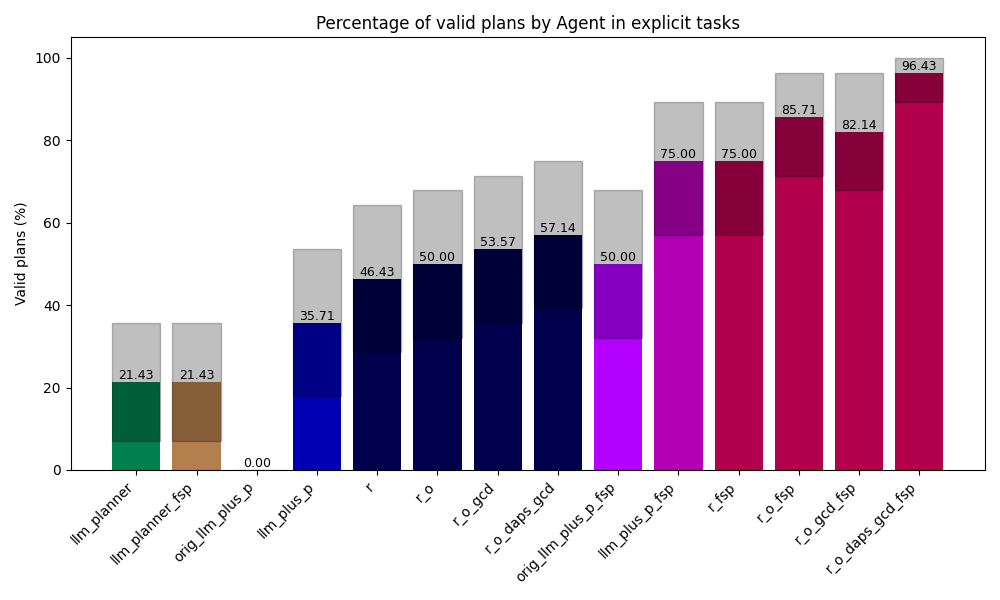
\includegraphics[width=0.7\textwidth]{Graphics/valid_plans_by_agent.png}
\caption{Porcentaje de planes válidos por agente en tareas con descripción completamente explícita.}
\label{fig:plans}
\end{figure}

A la izquierda se muestran los dos agentes planificadores reproducidos. A la derecha se presentan los agentes modeladores, organizados en dos grupos: los seis primeros no utilizan \textit{FSP}, mientras que los seis últimos sí lo hacen (indicados mediante barras en tonos más rojizos). Dentro de cada grupo, el orden corresponde a: agente original \textit{LLM+P}, reimplementación estructurada, y variantes con módulos adicionales. En todos los casos se sombrea el intervalo de confianza (IC) del 95\,\%.

Como se aprecia en la figura, ambos agentes planificadores generan planes válidos únicamente en el 21.43\,\% (IC: [7.14\,\%, 35.71\,\%]) de los problemas evaluados, es decir, 6 soluciones correctas. En cambio, todos los agentes modeladores ---con excepción de \texttt{orig\_llm\_plus\_p}--- superan ampliamente este resultado. Además, se observa una mejora progresiva en la métrica con la incorporación de los módulos propuestos. El agente que incluye todos los componentes alcanza el mejor desempeño, con una tasa de validez del 96.43\,\% (IC: [89.29\,\%, 100.00\,\%]), fallando solo en uno de los 28 problemas.

Estos resultados evidencian la complejidad del \textit{benchmark} Planetarium, que representa un reto considerable para agentes planificadores directos, y refuerzan la superioridad del enfoque basado en modelado explícito. Asimismo, proporcionan evidencia empírica del impacto positivo de los módulos de mejora propuestos, como antesala a los resultados globales que se presentan a continuación.

\section{Resultados generales}

En esta sección se presentan los resultados obtenidos por los distintos agentes modeladores evaluados sobre los 70 problemas del conjunto de prueba estratificado del \textit{benchmark Planetarium}, distribuidos en tres dominios: \textit{Blocksworld} (16 problemas), \textit{Gripper} (27 problemas) y \textit{Floor-Tile} (27 problemas). 

Se comparan 12 variantes de agentes: los agentes originales de \textit{LLM+P}, sus reimplementaciones estructuradas, y múltiples versiones incrementales mejoradas con los módulos propuestos en esta tesis. Las métricas consideradas incluyen: tasa de modelos con objetos correctamente identificados (\textit{Correct Objects count}), tasa de sintaxis válida (\textit{Parseable}), tasa de solubilidad (\textit{Solvable}) y tasa de problemas completamente correctos (\textit{Correct}). Cada métrica se expresa como porcentaje del total de problemas evaluados. Todos los intervalos de confianza (IC) presentados son del 95\,\%.

\subsection*{Tabla comparativa de métricas}

\begin{table}[H]
\centering
\label{tab:resultados_agentes}
\begin{tabular}{lcccc}
\toprule
\textbf{Agente} & \textbf{COC (\%)} & \textbf{Parseable (\%)} & \textbf{Solvable (\%)} & \textbf{Correct (\%)} \\
\midrule
\texttt{orig\_llm\_plus\_p} & \textcolor{red}{32.86} & \textcolor{red}{34.29} & \textcolor{red}{0.00} & \textcolor{red}{0.00} \\
\texttt{llm\_plus\_p} & 62.86 & \underline{87.14} & 54.29 & 22.86 \\
\texttt{r} & 62.86 & 82.86 & 62.86 & 30.00 \\
\texttt{r\_o} & \underline{95.71} & 84.29 & \underline{78.57} & \underline{42.86} \\
\texttt{r\_o\_gcd} & \textcolor{green!60!black}{98.57} & \underline{87.14} & 77.14 & \textcolor{green!60!black}{44.29} \\
\texttt{r\_o\_daps\_gcd} & 92.86 & \textcolor{green!60!black}{97.14} & \textcolor{green!60!black}{85.71} & 41.43 \\
\midrule
\texttt{orig\_llm\_plus\_p\_fsp} & \textbf{\textcolor{green!60!black}{100.00}} & \textcolor{red}{80.00} & \textcolor{red}{62.86} & \textcolor{red}{47.14} \\
\texttt{llm\_plus\_p\_fsp} & \textbf{\textcolor{green!60!black}{100.00}} & 87.14 & 82.86 & 57.14 \\
\texttt{r\_fsp} & \textbf{\textcolor{green!60!black}{100.00}} & 90.00 & 87.14 & 72.86 \\
\texttt{r\_o\_fsp} & \textbf{\textcolor{green!60!black}{100.00}} & 91.43 & \underline{88.57} & \underline{75.71} \\
\texttt{r\_o\_gcd\_fsp} & \textbf{\textcolor{green!60!black}{100.00}} & \underline{92.86} & \underline{88.57} & 67.14 \\
\texttt{r\_o\_daps\_gcd\_fsp} & \textbf{\textcolor{green!60!black}{100.00}} & \textbf{\textcolor{green!60!black}{100.00}} & \textbf{\textcolor{green!60!black}{94.29}} & \textbf{\textcolor{green!60!black}{81.43}} \\
\bottomrule
\end{tabular}
\caption{Resultados comparativos por agente modelador}
\end{table}

En la tabla anterior, los valores en \textcolor{green!60!black}{verde} indican el mejor resultado por métrica dentro de cada grupo (\textit{Zero-Shot} arriba y \textit{One-Shot} abajo), los \underline{subrayados} corresponden al segundo mejor valor, y los \textcolor{red}{rojos} representan el peor desempeño observado. En la tabla siguiente, de estas evaluaciones se destacan de igual manera los intervalos de confianza al 95\%.

\begin{table}[ht]
\centering
\small
\begin{tabular}{lcccc}
\toprule
\textbf{Agente} & \textbf{COC IC (\%)} & \textbf{Parseable IC (\%)} & \textbf{Solvable IC (\%)} & \textbf{Correct IC (\%)} \\
\midrule
\texttt{orig\_llm\_plus\_p} & \textcolor{red!70!black}{[22.86, 44.29]} & \textcolor{red!70!black}{[22.86, 45.71]} & \textcolor{red!70!black}{[0.00, 0.00]} & \textcolor{red!70!black}{[0.00, 0.00]} \\
\texttt{llm\_plus\_p} & [51.43, 74.29] & \underline{[78.57, 94.29]} & [42.86, 65.71] & [12.86, 32.86] \\
\texttt{r} & [51.43, 74.29] & [74.29, 91.43] & [51.43, 74.29] & [20.00, 41.43] \\
\texttt{r\_o} & \underline{[90.00, 100.00]} & [75.71, 92.86] & \underline{[68.57, 87.14]} & \underline{[31.43, 54.29]} \\
\texttt{r\_o\_gcd} & \textcolor{green!60!black}{[95.71, 100.00]} & \underline{[78.57, 94.29]} & [67.14, 87.14] & \textcolor{green!60!black}{[32.86, 55.71]} \\
\texttt{r\_o\_daps\_gcd} & [85.71, 98.57] & \textcolor{green!60!black}{[92.86, 100.00]} & \textcolor{green!60!black}{[77.14, 92.86]} & [30.00, 52.86] \\
\midrule
\texttt{orig\_llm\_plus\_p\_fsp} & \textbf{\textcolor{green!60!black}{[100.00, 100.00]}} & \textcolor{red!70!black}{[70.00, 88.57]} & \textcolor{red!70!black}{[51.43, 74.29]} & \textcolor{red!70!black}{[35.71, 58.57]} \\
\texttt{llm\_plus\_p\_fsp} & \textbf{\textcolor{green!60!black}{[100.00, 100.00]}} & [78.57, 94.29] & [74.29, 91.43] & [45.71, 68.57] \\
\texttt{r\_fsp} & \textbf{\textcolor{green!60!black}{[100.00, 100.00]}} & [82.86, 97.14] & [78.57, 94.29] & [61.43, 82.86] \\
\texttt{r\_o\_fsp} & \textbf{\textcolor{green!60!black}{[100.00, 100.00]}} & [84.29, 97.14] & \underline{[80.00, 95.71]} & \underline{[65.71, 85.71]} \\
\texttt{r\_o\_gcd\_fsp} & \textbf{\textcolor{green!60!black}{[100.00, 100.00]}} & \underline{[85.71, 98.57]} & \underline{[80.00, 95.71]} & [55.71, 78.57] \\
\texttt{r\_o\_daps\_gcd\_fsp} & \textbf{\textcolor{green!60!black}{[100.00, 100.00]}} & \textbf{\textcolor{green!60!black}{[100.00, 100.00]}} & \textbf{\textcolor{green!60!black}{[88.57, 98.57]}} & \textbf{\textcolor{green!60!black}{[71.43, 90.00]}} \\
\bottomrule
\end{tabular}
\caption{Intervalos de confianza al 95\% para cada métrica por agente.}
\label{tab:bootstrap_ic_agentes}
\end{table}


\subsection*{Gráficas comparativas}

\begin{figure}[H]
\centering
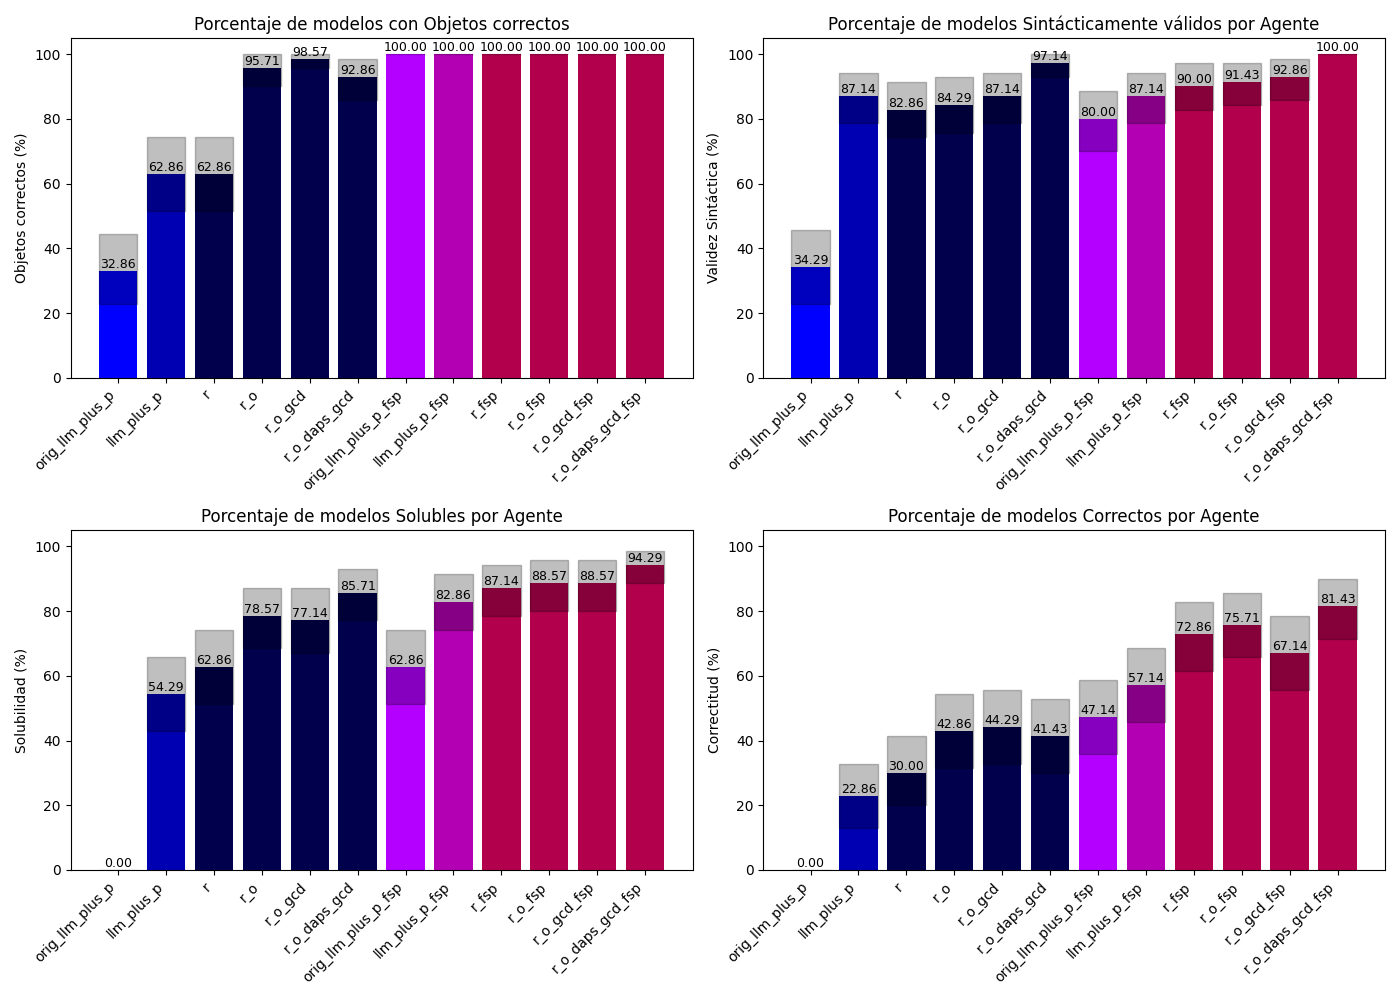
\includegraphics[width=0.8\textwidth]{Graphics/metrics_grid.png}
\caption{Métricas calculadas por agente}
\label{fig:objects}
\end{figure}

Estas gráficas de barras ilustran visualmente la evolución del desempeño de los agentes en cada una de las métricas clave. Los agentes se agrupan en dos bloques: los seis primeros no utilizan \textit{Few-Shot Prompting (FSP)}, mientras que los seis últimos sí lo hacen (indicados con barras en tonos más rojizos). En cada grupo, el orden de aparición sigue el patrón: agente original de \textit{LLM+P}, reimplementación estructurada, y variantes con módulos adicionales.

\subsection{Impacto del Razonamiento Estructurado}

El razonamiento estructurado fue incorporado como una fase previa y separada a la generación del modelo \textit{PDDL}, con el objetivo de descomponer semánticamente el problema y mejorar la calidad del modelado automático. Esta etapa adicional fue diseñada para inducir al \textit{LLM} a procesar explícitamente los objetos, el estado inicial y el estado objetivo antes de generar la solución final.

El impacto de este componente puede analizarse con claridad a partir de comparaciones directas entre agentes que difieren únicamente en la presencia del razonamiento. Por ejemplo, al comparar \texttt{llm\_plus\_p} con \texttt{r}, se observa una mejora en la proporción de modelos solubles, que aumenta de 54.29\,\% (IC: [42.86\,\%, 65.71\,\%]) a 62.86\,\% (IC: [51.43\,\%, 74.29\,\%]), así como en la proporción de problemas \textit{correctos}, que pasa de 22.86\,\% (IC: [12.86\,\%, 32.86\,\%]) a 30.00\,\% (IC: [20.00\,\%, 41.43\,\%]). Aunque los intervalos de confianza se superponen, la diferencia observada indica un efecto positivo consistente del componente, atribuible al cambio en la estrategia cognitiva del agente.

La comparación en presencia de \textit{Few-Shot Prompting (FSP)} ofrece aún mayor contraste. Al comparar \texttt{llm\_plus\_p\_fsp} con \texttt{r\_fsp}, se aprecia un aumento en la métrica de solubilidad de 82.86\,\% (IC: [74.29\,\%, 91.43\,\%]) a 87.14\,\% (IC: [78.57\,\%, 94.29\,\%]), y en la de \textit{correctitud completa} de 57.14\,\% (IC: [45.71\,\%, 68.57\,\%]) a 72.86\,\% (IC: [61.43\,\%, 82.86\,\%]). Esta diferencia es significativa tanto en magnitud como en intervalo de confianza, y puede explicarse por el hecho de que los ejemplos de \textit{FSP} fueron cuidadosamente diseñados para mostrar razonamientos y desambiguaciones correctas, lo que actúa como una guía concreta para que el \textit{LLM} aprenda cómo estructurar sus propias inferencias sobre tareas de planificación.

Los beneficios del razonamiento no se extienden a las métricas de \textit{objetos correctos} y \textit{modelo con sintaxis válida}, pero no tiene un efecto negativo palpable. Por ejemplo, entre \texttt{llm\_plus\_p} y \texttt{r}, la proporción de objetos correctamente identificados se mantiene constante en 62.86\,\% (IC: [51.43\,\%, 74.29\,\%]), lo cual sugiere que este componente no deteriora la precisión de este aspecto, mientras que la validez sintáctica se mantiene elevada (de 87.14\,\% (IC: [78.57\,\%, 94.29\,\%]) a 82.86\,\% (IC: [74.29\,\%, 91.43\,\%])), aunque con una ligera caída en la media. Estas fluctuaciones pueden deberse a alucinaciones, que en ausencia de ejemplos de \textit{FSP} y razonamiento ineficiente pueden acentuarse. Más aún, se observa que la validez sintáctica aumenta ligeramente en el par de agentes \textit{One-Shot}, de 87.14\,\% (IC: [78.57\,\%, 94.29\,\%]) a 90.00\,\% (IC: [82.86\,\%, 97.14\,\%]). Sin embargo, estos resultados no son concluyentes y no comprometen la interpretación general.

Cabe destacar que, debido al diseño incremental del sistema, los resultados de los agentes más avanzados (como \texttt{r\_o\_gcd} o \texttt{r\_o\_daps\_gcd}) reflejan interacciones acumulativas entre múltiples componentes. Por tanto, el impacto aislado del razonamiento estructurado debe analizarse principalmente en los pares donde es el único cambio introducido. Aun así, su presencia constante en los agentes de mayor rendimiento (tanto con como sin \textit{FSP}) sugiere que su efecto es no solo positivo, sino posiblemente sinérgico con otros módulos.

Estos resultados empíricos se alinean con hallazgos previos en la literatura, que indican que la inclusión de pasos intermedios de razonamiento mejora las capacidades de los \textit{LLMs} en tareas complejas \parencite{wei2022chain, yao2023tree}. En particular, trabajos como \textit{ReAct} \parencite{yao2023react} han demostrado que combinar razonamiento textual con ejecución no solo mejora la calidad de las salidas, sino que también aumenta la interpretabilidad del proceso. Los resultados obtenidos en esta tesis refuerzan dicha hipótesis, mostrando que una etapa explícita de razonamiento puede traducirse en mejoras cuantificables en desempeño y robustez del agente modelador.

\subsection{Impacto de la Extracción de Objetos}

La Extracción de Objetos se incorporó como una etapa estructurada y especializada con el objetivo de mejorar la precisión semántica y sintáctica del modelo \textit{PDDL} generado. Al separar explícitamente la identificación de objetos relevantes del resto del proceso, se busca garantizar la integridad del conjunto de elementos que participan en el problema de planificación. Esta fase se implementó posterior al razonamiento (cuando está activo), permitiendo heredar y organizar las inferencias previas, y su salida se genera en un formato \textit{JSON} que facilita su uso posterior en componentes como la generación asistida por gramática (\textit{GCD}).

Desde el punto de vista empírico, el impacto de este componente puede observarse de forma clara al comparar agentes que difieren únicamente en la presencia de esta fase. El caso más representativo es el contraste entre \texttt{r} y \texttt{r\_o}, donde se mantiene el razonamiento estructurado y se añade únicamente la extracción de objetos. En esta comparación, la proporción de objetos correctamente identificados aumenta de 62.86\,\% (IC: [51.43\,\%, 74.29\,\%]) a 95.71\,\% (IC: [90.00\,\%, 100.00\,\%]), lo cual representa una mejora sustancial en el componente más directamente afectado por esta fase.

Además, esta mejora en la identificación de objetos se traduce en ganancias indirectas en otras métricas. La validez sintáctica se mantiene estable, con un ligero aumento de 82.86\,\% (IC: [74.29\,\%, 91.43\,\%]) a 84.29\,\% (IC: [75.71\,\%, 92.86\,\%]). La solubilidad mejora sustancialmente, de 62.86\,\% (IC: [51.43\,\%, 74.29\,\%]) a 78.57\,\% (IC: [68.57\,\%, 87.14\,\%]). En correctitud total, \texttt{r} alcanza 30.00\,\% (IC: [20.00\,\%, 41.43\,\%]), mientras que \texttt{r\_o} sube a 42.86\,\% (IC: [31.43\,\%, 54.29\,\%]). Esto sugiere que la correcta extracción y estructuración de objetos permite al modelo generar instancias más completas y coherentes, impactando positivamente tanto en la validez sintáctica como semántica.

Un patrón similar se repite en los agentes que incorporan \textit{FSP}. Comparando \texttt{r\_fsp} y \texttt{r\_o\_fsp}, se observa una mejora en solubilidad de 87.14\,\% (IC: [78.57\,\%, 94.29\,\%]) a 88.57\,\% (IC: [80.00\,\%, 95.71\,\%]), así como una ganancia en correctitud total de 72.86\,\% (IC: [61.43\,\%, 82.86\,\%]) a 75.71\,\% (IC: [65.71\,\%, 85.71\,\%]). Aunque estas diferencias son más sutiles, reflejan una consolidación de los beneficios observados en el grupo sin \textit{FSP}.

Estas observaciones refuerzan la utilidad de una fase de extracción dedicada, especialmente en contextos donde la ambigüedad o la omisión de objetos puede deteriorar gravemente la calidad del modelo generado. Al permitir una representación explícita, detallada y consistente de los objetos del dominio, este componente actúa como un estabilizador semántico clave que fortalece las fases posteriores del \textit{pipeline} de modelado.

Finalmente, es importante señalar que este módulo facilita no solo la calidad de los modelos, sino también su inspeccionabilidad y adaptabilidad. Su diseño como fase independiente y estructurada habilita un nivel adicional de trazabilidad que puede ser aprovechado tanto para depuración como para transferencia de conocimiento entre tareas similares, especialmente cuando se combina con componentes como \textit{GCD} o reflexión estructurada. Permite, más aún, la aplicación de la modalidad \textit{DAPS} concebida de \textit{GCD}, al restringir la salida del modelo a una gramática específica al problema a modelar, limitando los argumentos utilizados en las proposiciones a aquellos objetos extraídos en esta fase, con correcto tipado si lo presentan.

\subsection{Impacto de \textit{Grammar-Constrained Decoding (GCD)} y su variante \textit{Domain-and Problem-Specific (DAPS)}}

El módulo de \textit{GCD} fue introducido con el objetivo de garantizar la validez sintáctica de los modelos \textit{PDDL} generados, mediante la incorporación de una gramática explícita sobre la estructura del lenguaje. Como punto de partida, se utilizó una gramática en formato \textit{GBNF} que captura la sintaxis del subconjunto de \textit{PDDL} empleado, incluyendo soporte para dominios tipados y la estructura general de \textit{STRIPS}. Esta gramática permite restringir la generación a secuencias sintácticamente válidas, pero no impone restricciones semánticas específicas al dominio o problema en cuestión.

Para superar estas limitaciones, se introdujo una variante más estricta denominada \textit{Domain-and Problem-Specific (DAPS)}, la cual incorpora de forma dinámica los predicados, tipos y objetos específicos del problema en curso. En particular, se especializa la producción de fórmulas atómicas dentro de las secciones \texttt{:init} y \texttt{:goal}, de modo que solo se aceptan predicados válidos del dominio, con aridad exacta y argumentos seleccionados exclusivamente del conjunto de objetos declarados. Esto impide que el modelo produzca contenido fuera del esquema válido, como razonamientos embebidos o correcciones autorreferenciales dentro de estructuras que requieren literalidad.

Un ejemplo de este comportamiento problemático puede verse en la producción básica de fórmulas atómicas sin restricciones específicas:

\begin{verbatim}
atomicFormula ::= "(" name (ws object)* ")"
\end{verbatim}

Esta definición permite que casi cualquier secuencia de texto sea interpretada como el nombre de un predicado o un argumento, lo que en la práctica genera errores de sintaxis, especialmente cuando el \textit{LLM} introduce razonamientos o comentarios no deseados dentro de las proposiciones. En contraste, en la modalidad \textit{DAPS} se sustituye esta producción por una versión especializada que considera únicamente combinaciones válidas y completas de predicado y argumentos.

En términos empíricos, el impacto de \textit{GCD} puede observarse en el paso de \texttt{r\_o} a \texttt{r\_o\_gcd}, donde se mantiene el razonamiento y la extracción de objetos, pero se añade el uso de la gramática general. La validez sintáctica mejora de 84.29\,\% (IC: [75.71\,\%, 92.86\,\%]) a 87.14\,\% (IC: [78.57\,\%, 94.29\,\%]), lo cual muestra una ganancia modesta, posiblemente limitada por las desviaciones mencionadas. Estas también afectan la solubilidad, donde se observa un ligero descenso, de 78.57\,\% (IC: [68.57\,\%, 87.14\,\%]) a 77.14\,\% (IC: [67.14\,\%, 87.14\,\%]), aunque no es estadísticamente significativo considerando la intersección casi total de los intervalos de confianza. La correctitud total sube levemente de 42.86\,\% (IC: [31.43\,\%, 54.29\,\%]) a 44.29\,\% (IC: [32.86\,\%, 55.71\,\%]).

Sin embargo, la modalidad \textit{DAPS} muestra una mejora mucho más marcada. En \texttt{r\_o\_daps\_gcd}, se observa que la validez sintáctica alcanza el 97.14\,\% (IC: [92.86\,\%, 100.00\,\%]). También se reporta un aumento significativo en solubilidad, a 85.71\,\% (IC: [77.14\,\%, 92.86\,\%]), aunque esta mejora no se observa en la correctitud, posiblemente por la ausencia en el contexto de buenos ejemplos de razonamiento estructurado. Estos resultados respaldan empíricamente la hipótesis de que una gramática altamente especializada aporta grandes beneficios en la validez sintáctica de los modelos.

Este efecto se ve reforzado cuando se analiza la interacción con \textit{Few-Shot Prompting (FSP)}. En el caso del agente \texttt{r\_o\_fsp}, que ya alcanza valores altos en todas las métricas, se obtiene una validez sintáctica de 91.43\,\% (IC: [84.29\,\%, 97.14\,\%]), una \textit{solubilidad} de 88.57\,\% (IC: [80.00\,\%, 95.71\,\%]) y una \textit{correctitud total} de 75.71\,\% (IC: [65.71\,\%, 85.71\,\%]). Al incorporar la gramática general mediante \texttt{GCD} en \texttt{r\_o\_gcd\_fsp}, la validez sintáctica mejora levemente a 92.86\,\% (IC: [85.71\,\%, 98.57\,\%]), y la solubilidad se mantiene constante, aunque la correctitud total disminuye a 67.14\,\% (IC: [55.71\,\%, 78.57\,\%]), probablemente debido a las desviaciones observadas por control gramatical y semántico incompleto. Finalmente, al incorporar la modalidad \textit{DAPS} en \texttt{r\_o\_daps\_gcd\_fsp}, se logra validez sintáctica perfecta (100\,\%, IC: [100\,\%, 100\,\%]), una solubilidad de 94.29\,\% (IC: [88.57\,\%, 98.57\,\%]) y una correctitud total de 81.43\,\% (IC: [71.43\,\%, 90.00\,\%]), lo cual representa el mejor desempeño alcanzado por cualquier agente evaluado en todas las métricas, con una diferencia marcada.

Cabe señalar que, pese a la formalización gramatical, la modalidad \textit{GCD} no garantiza validez sintáctica perfecta por sí sola. Esto se debe a que las gramáticas generales no impiden por completo que el \textit{LLM} inserte contenido erróneo o se desvíe del formato literal requerido, como ocurre al generar proposiciones en \texttt{:init} y \texttt{:goal}. Solo mediante la especialización del conjunto de producciones a través de \textit{DAPS} se evita completamente este comportamiento.

Estos hallazgos empíricos respaldan las observaciones de trabajos previos como \parencite{loula2025syntactic}, que demostraban el potencial de \textit{GCD} para mejorar la coherencia sintáctica en dominios acotados. Sin embargo, la evaluación presentada en esta tesis extiende significativamente dicho análisis al considerar la generación completa de modelos \textit{PDDL} a partir de descripciones en lenguaje natural y una evaluación exhaustiva sobre un subconjunto estratificado de problemas más representativo del \textit{benchmark Planetarium}. Además, se introduce y valida empíricamente un refinamiento fundamental: la especialización semántica de la gramática con base en el dominio y problema, lo cual constituye un avance práctico y conceptual en el uso de \textit{GCD} para modelado automático en planificación.

\subsection{Un salto cualitativo sobre los \textit{baselines} existentes}

Para ilustrar la magnitud del avance logrado por la variante \texttt{r\_o\_daps\_gcd\_fsp}, es fundamental contrastarla con los \textit{baselines} \texttt{orig\_llm\_plus\_p\_fsp} y \texttt{llm\_plus\_p\_fsp}. En validez sintáctica, los valores de 80.00\,\% y 87.14\,\% alcanzados por los respectivos \textit{baselines} son completamente superados: \texttt{r\_o\_daps\_gcd\_fsp} logra una cobertura total del 100\,\%, cerrando el 100\,\% del margen restante en ambos casos. 

En solubilidad, la mejora es igualmente destacable. \texttt{orig\_llm\_plus\_p\_fsp} alcanzaba 62.86\,\%, quedando un 37.14\,\% por recorrer; \texttt{r\_o\_daps\_gcd\_fsp} logra 94.29\,\%, salvando 31.43 puntos, lo que equivale a un 84.63\,\% de ese margen. Similarmente, frente al 82.86\,\% de \texttt{llm\_plus\_p\_fsp}, que dejaba 17.14\,\% por cubrir, \texttt{r\_o\_daps\_gcd\_fsp} salva 11.43 puntos, un 66.67\,\% del margen de mejora.

La diferencia es aún más relevante en \textit{correctitud total}, la métrica más exigente e importante. En ella \texttt{orig\_llm\_plus\_p\_fsp} obtenía 47.14\,\% (quedando un 52.86\,\% restante), y \texttt{r\_o\_daps\_gcd\_fsp} alcanza 81.43\,\%, cubriendo 34.29 puntos, un 64.86\,\% del espacio disponible. Frente a \texttt{llm\_plus\_p\_fsp} (57.14\,\%), que dejaba 42.86\,\% por salvar, la misma variante logra cubrir 24.29 puntos, es decir un 56.67\,\% de dicho faltante. Dicho de otro modo, más de la mitad de lo que los agentes anteriores no lograban modelar correctamente, es resuelto por la variante que aplica todas las mejoras propuestas.

Estos cálculos muestran que, más allá de la diferencia absoluta en puntos porcentuales, la combinación de \textit{GCD} especializada (\textit{DAPS}) con \textit{FSP} manual, mecanismos de \textit{extracción de objetos} consistentes, y el uso explícito de \textit{razonamiento estructurado}, proporciona una mejora \textbf{proporcionalmente muy significativa} sobre lo que faltaba en los \textit{baselines}. Estos resultados demuestran empíricamente el potencial de los componentes propuestos actuando en conjunto para cerrar brechas que los enfoques anteriores apenas lograban mitigar.

\definecolor{verde}{HTML}{008000} % Define el color verde
\definecolor{rojo}{HTML}{FF0000} % Define el color rojo

\section{Entrenamiento del agente modelador experiencial}

Se llevó a cabo el entrenamiento propuesto del agente modelador experiencial sobre el subconjunto seleccionado de 100 problemas, 50 del dominio \textit{Blocksworld} y 50 del dominio \textit{Gripper}. El agente implementó la configuración \texttt{r\_o\_daps\_gcd\_fsp}, incorporando los módulos de Razonamiento Estructurado, Extracción de Objetos, \textit{GCD DAPS} y un ejemplo \textit{FSP} definido manualmente, representando así la mejor versión evaluada en iteraciones anteriores. Además, se integró el mecanismo de reintentos, que permitía al agente iterar hasta tres veces sobre cada problema, guiado por \textit{feedback} automático y autorreflexión para mejorar su rendimiento. El agente resultante será denominado \texttt{exp} por simplicidad.

La tabla que se presenta a continuación resume los resultados de este proceso de entrenamiento. Cada fila corresponde a una configuración particular de resultados a través de los tres intentos permitidos por problema. Para cada intento, se registran tres las métricas definidas anteriormente: \textit{Parseable} ($\mathcal{P}$), \textit{Solvable} ($\mathcal{S}$) y \textit{Correct} ($\mathcal{C}$). Una \textcolor{verde}{\textbf{V}} representa un resultado positivo, mientras que una \textcolor{rojo}{\textbf{F}} indica un resultado negativo para esa métrica en ese intento. El índice numérico en cada métrica indica el intento (ej., $\mathcal{P}_1$ corresponde a la validez sintáctica en el primer intento). La última columna, ``Número de Problemas'', indica la cantidad de problemas que determinaron esa secuencia específica de resultados a lo largo de los intentos del agente.

\begin{table}[h!]
    \centering
    \caption{Resultados del Agente en Problemas de Planificación}
    \begin{tabular}{ccc@{\hspace{2em}}ccc@{\hspace{2em}}ccc@{\hspace{2em}}c}
        \toprule
        \multicolumn{3}{c}{\textbf{Intento 1}} & \multicolumn{3}{c}{\textbf{Intento 2}} & \multicolumn{3}{c}{\textbf{Intento 3}} & \textbf{Número de Problemas} \\
        \cmidrule(lr){1-3} \cmidrule(lr){4-6} \cmidrule(lr){7-9}
        $\mathcal{P}_1$ & $\mathcal{S}_1$ & $\mathcal{C}_1$ & $\mathcal{P}_2$ & $\mathcal{S}_2$ & $\mathcal{C}_2$ & $\mathcal{P}_3$ & $\mathcal{S}_3$ & $\mathcal{C}_3$ & \\
        \midrule
        \textcolor{verde}{\textbf{V}} & \textcolor{verde}{\textbf{V}} & \textcolor{verde}{\textbf{V}} & - & - & - & - & - & - & 87 \\
        \textcolor{verde}{\textbf{V}} & \textcolor{verde}{\textbf{V}} & \textcolor{rojo}{\textbf{F}} & \textcolor{verde}{\textbf{V}} & \textcolor{verde}{\textbf{V}} & \textcolor{verde}{\textbf{V}} & - & - & - & 2 \\
        \textcolor{verde}{\textbf{V}} & \textcolor{verde}{\textbf{V}} & \textcolor{rojo}{\textbf{F}} & \textcolor{verde}{\textbf{V}} & \textcolor{verde}{\textbf{V}} & \textcolor{rojo}{\textbf{F}} & \textcolor{verde}{\textbf{V}} & \textcolor{verde}{\textbf{V}} & \textcolor{verde}{\textbf{V}} & 1 \\
        \textcolor{verde}{\textbf{V}} & \textcolor{verde}{\textbf{V}} & \textcolor{rojo}{\textbf{F}} & \textcolor{verde}{\textbf{V}} & \textcolor{verde}{\textbf{V}} & \textcolor{rojo}{\textbf{F}} & \textcolor{verde}{\textbf{V}} & \textcolor{verde}{\textbf{V}} & \textcolor{rojo}{\textbf{F}} & 2 \\
        \textcolor{verde}{\textbf{V}} & \textcolor{rojo}{\textbf{F}} & \textcolor{rojo}{\textbf{F}} & \textcolor{verde}{\textbf{V}} & \textcolor{verde}{\textbf{V}} & \textcolor{verde}{\textbf{V}} & - & - & - & 4 \\
        \textcolor{verde}{\textbf{V}} & \textcolor{rojo}{\textbf{F}} & \textcolor{rojo}{\textbf{F}} & \textcolor{verde}{\textbf{V}} & \textcolor{rojo}{\textbf{F}} & \textcolor{rojo}{\textbf{F}} & \textcolor{verde}{\textbf{V}} & \textcolor{verde}{\textbf{V}} & \textcolor{verde}{\textbf{V}} & 1 \\
        \textcolor{verde}{\textbf{V}} & \textcolor{rojo}{\textbf{F}} & \textcolor{rojo}{\textbf{F}} & \textcolor{verde}{\textbf{V}} & \textcolor{rojo}{\textbf{F}} & \textcolor{rojo}{\textbf{F}} & \textcolor{verde}{\textbf{V}} & \textcolor{rojo}{\textbf{F}} & \textcolor{rojo}{\textbf{F}} & 1 \\
        \textcolor{rojo}{\textbf{F}} & \textcolor{rojo}{\textbf{F}} & \textcolor{rojo}{\textbf{F}} & \textcolor{verde}{\textbf{V}} & \textcolor{verde}{\textbf{V}} & \textcolor{verde}{\textbf{V}} & - & - & - & 1 \\
        \textcolor{rojo}{\textbf{F}} & \textcolor{rojo}{\textbf{F}} & \textcolor{rojo}{\textbf{F}} & \textcolor{verde}{\textbf{V}} & \textcolor{rojo}{\textbf{F}} & \textcolor{rojo}{\textbf{F}} & \textcolor{verde}{\textbf{V}} & \textcolor{verde}{\textbf{V}} & \textcolor{verde}{\textbf{V}} & 1 \\
        \bottomrule
    \end{tabular}
    \label{tab:entrenamiento}
\end{table}

Los resultados revelan una alta tasa de éxito en el primer intento, con 87 problemas siendo resueltos correctamente de inmediato. Sin embargo, la inclusión del mecanismo de reintentos demostró ser crucial para mejorar el rendimiento general. Si bien algunos problemas presentaron dificultades persistentes a lo largo de los tres intentos, la autorreflexión y el \textit{feedback} automático permitieron al agente corregir errores y alcanzar soluciones completamente correctas en intentos posteriores para 10 de los 13 problemas inicialmente fallidos. De los 3 problemas cuyo modelado no fue correcto en ninguno de los intentos, 2 resultaron solubles. Contando únicamente los primeros intentos por cada problema, se alcanzaban tasas de validez sintáctica de 98 \% (debido a truncamientos de la salida del \textit{LLM}), 92 \% de solubilidad y 87 \% de correctitud. Finalmente, con la integración de los reintentos, el agente \texttt{exp} alcanzó en el entrenamiento una validez sintáctica del 100 \%, solubilidad del 99 \%, y 97 \% de correctitud. Este análisis sugiere que la combinación de capacidades de modelado robustas con mecanismos adaptativos de auto-mejora contribuye significativamente a la capacidad del agente para abordar una amplia gama de desafíos de planificación.

\section{Aplicación de reintentos, \textit{feedback} y reflexión a la evaluación}

El agente \texttt{exp} aplicó la política de reintentos definida anteriormente a los problemas modelados incorrectamente por el agente \texttt{r\_o\_daps\_gcd\_fsp}, sobre el subconjunto de evaluación. Las salidas (razonamiento, objetos extraídos y \textit{PDDL} del problema) generados en su primer y único intento por tarea, y el \textit{feedback} construido automáticamente sobre este fallo, contribuyeron a un segundo intento que incluyó reflexión sobre la retroalimentación dada. De igual forma, se permitió un tercer intento apoyado en los resultados del segundo, si este era incorrecto.

La evaluación de \texttt{exp} se resume en la tabla siguiente:

\begin{table}[h!]
    \centering
    \caption{Resultados del Agente en el conjunto de Evaluación}
    \begin{tabular}{ccc@{\hspace{2em}}ccc@{\hspace{2em}}ccc@{\hspace{2em}}c}
        \toprule
        \multicolumn{3}{c}{\textbf{Intento 1}} & \multicolumn{3}{c}{\textbf{Intento 2}} & \multicolumn{3}{c}{\textbf{Intento 3}} & \textbf{Número de Problemas} \\
        \cmidrule(lr){1-3} \cmidrule(lr){4-6} \cmidrule(lr){7-9}
        $\mathcal{P}_1$ & $\mathcal{S}_1$ & $\mathcal{C}_1$ & $\mathcal{P}_2$ & $\mathcal{S}_2$ & $\mathcal{C}_2$ & $\mathcal{P}_3$ & $\mathcal{S}_3$ & $\mathcal{C}_3$ & \\
        \midrule
        \textcolor{verde}{\textbf{V}} & \textcolor{verde}{\textbf{V}} & \textcolor{verde}{\textbf{V}} & - & - & - & - & - & - & 57 \\
        \textcolor{verde}{\textbf{V}} & \textcolor{verde}{\textbf{V}} & \textcolor{rojo}{\textbf{F}} & \textcolor{verde}{\textbf{V}} & \textcolor{verde}{\textbf{V}} & \textcolor{rojo}{\textbf{F}} & \textcolor{verde}{\textbf{V}} & \textcolor{verde}{\textbf{V}} & \textcolor{rojo}{\textbf{F}} & 5 \\
        \textcolor{verde}{\textbf{V}} & \textcolor{verde}{\textbf{V}} & \textcolor{rojo}{\textbf{F}} & \textcolor{verde}{\textbf{V}} & \textcolor{verde}{\textbf{V}} & \textcolor{rojo}{\textbf{F}} & \textcolor{rojo}{\textbf{F}} & \textcolor{rojo}{\textbf{F}} & \textcolor{rojo}{\textbf{F}} & 2 \\
        \textcolor{verde}{\textbf{V}} & \textcolor{verde}{\textbf{V}} & \textcolor{rojo}{\textbf{F}} & \textcolor{verde}{\textbf{V}} & \textcolor{rojo}{\textbf{F}} & \textcolor{rojo}{\textbf{F}} & \textcolor{verde}{\textbf{V}} & \textcolor{verde}{\textbf{V}} & \textcolor{rojo}{\textbf{F}} & 1 \\
        \textcolor{verde}{\textbf{V}} & \textcolor{verde}{\textbf{V}} & \textcolor{rojo}{\textbf{F}} & \textcolor{rojo}{\textbf{F}} & \textcolor{rojo}{\textbf{F}} & \textcolor{rojo}{\textbf{F}} & \textcolor{verde}{\textbf{V}} & \textcolor{verde}{\textbf{V}} & \textcolor{rojo}{\textbf{F}} & 1 \\
        \textcolor{verde}{\textbf{V}} & \textcolor{rojo}{\textbf{F}} & \textcolor{rojo}{\textbf{F}} & \textcolor{verde}{\textbf{V}} & \textcolor{verde}{\textbf{V}} & \textcolor{rojo}{\textbf{F}} & \textcolor{verde}{\textbf{V}} & \textcolor{verde}{\textbf{V}} & \textcolor{verde}{\textbf{V}} & 2 \\
        \textcolor{verde}{\textbf{V}} & \textcolor{rojo}{\textbf{F}} & \textcolor{rojo}{\textbf{F}} & \textcolor{verde}{\textbf{V}} & \textcolor{verde}{\textbf{V}} & \textcolor{rojo}{\textbf{F}} & \textcolor{verde}{\textbf{V}} & \textcolor{rojo}{\textbf{F}} & \textcolor{rojo}{\textbf{F}} & 1 \\
        \textcolor{verde}{\textbf{V}} & \textcolor{rojo}{\textbf{F}} & \textcolor{rojo}{\textbf{F}} & \textcolor{verde}{\textbf{V}} & \textcolor{rojo}{\textbf{F}} & \textcolor{rojo}{\textbf{F}} & \textcolor{verde}{\textbf{V}} & \textcolor{rojo}{\textbf{F}} & \textcolor{rojo}{\textbf{F}} & 1 \\
        \bottomrule
    \end{tabular}
    \label{tab:eval_con_reintentos}
\end{table}

Los resultados obtenidos en la evaluación son menos alentadores que los del entrenamiento. En general, el agente con reflexión (\texttt{exp}) mostró dificultades para mejorar su desempeño, e incluso en algunos casos obtuvo resultados inferiores en reintentos. Esto podría atribuirse a la mayor complejidad inherente a los problemas no resueltos, que frecuentemente involucraban modelos \textit{PDDL} con un centenar de proposiciones. Los reintentos se caracterizaron por dos factores que afectaron negativamente al agente: un contexto mucho más extenso, influenciado por las salidas previas, y una reflexión propensa a alucinaciones. La degradación del rendimiento de los \textit{LLMs} con contextos extensos es un fenómeno bien documentado \parencite{li2024long}. Esta problemática se exacerbó en los problemas del dominio \textit{Floor-Tile}, ausente en el conjunto de entrenamiento anteriormente analizado. Este dominio requiere múltiples proposiciones para definir explícitamente la adyacencia entre celdas, utilizando predicados como \texttt{(up tileX tileY)} y \texttt{(right tileX tileY)}.  Con frecuencia, el agente alucinaba la existencia y necesidad de predicados similares como \texttt{left} y \texttt{down}. Aunque estos predicados no son permitidos por la restricción gramatical implementada con \textit{DAPS GCD}, su alucinación en la reflexión o razonamiento constituye ruido que dificulta el modelado correcto.

A pesar de estos resultados iniciales, el potencial de los mecanismos propuestos no debe descartarse. De los 13 problemas que el agente no logró modelar correctamente en el intento inicial de la etapa de evaluación, se corrigieron 2 gracias a los reintentos. La evaluación inicial ya mostraba resultados elevados, con un 100\,\% de validez sintáctica, un 94.29\,\% de solubilidad y un 81.43\,\% de correctitud, con dificultad de mejoría. Sin embargo, al considerar el mejor resultado obtenido en los reintentos para cada problema, estas métricas se incrementan a 100\,\%, 98.57\,\% y 84.29\,\%, respectivamente.

\section{Extracción de \textit{insights}}

La fase de extracción de \textit{insights}, posterior a la acumulación de experiencias durante el entrenamiento, se llevó a cabo de forma exploratoria. Sin embargo, los resultados iniciales no fueron del todo satisfactorios. Los \textit{insights} generados por el \textit{LLM}, actuando como agente extractor, tendían a ser vagos, genéricos o poco relevantes. En muchos casos, no lograban captar conocimiento concreto o útil del dominio que pudiera contribuir de forma significativa al modelado de nuevos problemas.

Además, las respuestas del modelo presentaban divagaciones extensas, con escasa alineación a las operaciones válidas del entorno, y sin un control efectivo sobre las restricciones sintácticas y semánticas de las acciones. Esto generó dificultades importantes para el análisis automático de las salidas, afectando la robustez del procesamiento posterior y provocando errores de ejecución en algunos casos. Estos comportamientos apuntan a posibles deficiencias en la ingeniería de \textit{prompts}, particularmente en su capacidad para guiar al modelo hacia la identificación de patrones estructurados y reutilizables de conocimiento relevante.

\section{Evaluación del agente experiencial con todos los módulos incluidos}

En la fase final de experimentación se evaluó el agente modelador completo, que integra todos los componentes diseñados en esta tesis para mejorar progresivamente los resultados. Este agente experiencial, reforzado con ejemplos derivados de experiencias anteriores, incorpora módulos de recuperación de ejemplos vía \textit{RAG} y conocimiento experto curado manualmente.

En concreto, se reutilizaron los ejemplos de \textit{FSP} aprendidos durante la fase de entrenamiento para los dominios \textit{Blocksworld} y \textit{Gripper}, recuperados automáticamente mediante \textit{RAG}. Para el dominio \textit{Floor-Tile}, sin instancias incluidas en el entrenamiento, se empleó el ejemplo construido manualmente.

Dado el rendimiento limitado observado en la extracción automática de \textit{insights}, se diseñó y empleó una base de \textit{Human Insights} (HI) creada manualmente. Esta decisión permite evaluar el impacto de integrar conocimiento estructurado y explícito, extraído por un experto humano, en lugar de depender exclusivamente de la inferencia del modelo, cuya mejora se delega a trabajo futuro.

El agente evaluado, denominado \texttt{exp\_rag\_hi}, combina así dos mecanismos de conocimiento experiencial: \textit{Retrieval-Augmented Generation} (RAG) y \textit{Human Insights} (HI). Los resultados obtenidos se presentan a continuación.

\begin{table}[H]
    \centering
    \caption{Resultados en el conjunto completo de evaluación}
    \begin{tabular}{ccc@{\hspace{2em}}ccc@{\hspace{2em}}ccc@{\hspace{2em}}c}
        \toprule
        \multicolumn{3}{c}{\textbf{Intento 1}} & \multicolumn{3}{c}{\textbf{Intento 2}} & \multicolumn{3}{c}{\textbf{Intento 3}} & \textbf{Número de Problemas} \\
        \cmidrule(lr){1-3} \cmidrule(lr){4-6} \cmidrule(lr){7-9}
        $\mathcal{P}_1$ & $\mathcal{S}_1$ & $\mathcal{C}_1$ & $\mathcal{P}_2$ & $\mathcal{S}_2$ & $\mathcal{C}_2$ & $\mathcal{P}_3$ & $\mathcal{S}_3$ & $\mathcal{C}_3$ & \\
        \midrule
        \textcolor{verde}{\textbf{V}} & \textcolor{verde}{\textbf{V}} & \textcolor{verde}{\textbf{V}} & - & - & - & - & - & - & 57 \\
        \textcolor{verde}{\textbf{V}} & \textcolor{verde}{\textbf{V}} & \textcolor{rojo}{\textbf{F}} & \textcolor{verde}{\textbf{V}} & \textcolor{verde}{\textbf{V}} & \textcolor{verde}{\textbf{V}} & - & - & - & 1 \\
        \textcolor{verde}{\textbf{V}} & \textcolor{verde}{\textbf{V}} & \textcolor{rojo}{\textbf{F}} & \textcolor{verde}{\textbf{V}} & \textcolor{verde}{\textbf{V}} & \textcolor{rojo}{\textbf{F}} & \textcolor{verde}{\textbf{V}} & \textcolor{verde}{\textbf{V}} & \textcolor{verde}{\textbf{V}} & 1 \\
        \textcolor{verde}{\textbf{V}} & \textcolor{verde}{\textbf{V}} & \textcolor{rojo}{\textbf{F}} & \textcolor{verde}{\textbf{V}} & \textcolor{verde}{\textbf{V}} & \textcolor{rojo}{\textbf{F}} & \textcolor{verde}{\textbf{V}} & \textcolor{verde}{\textbf{V}} & \textcolor{rojo}{\textbf{F}} & 8 \\
        \textcolor{verde}{\textbf{V}} & \textcolor{verde}{\textbf{V}} & \textcolor{rojo}{\textbf{F}} & \textcolor{verde}{\textbf{V}} & \textcolor{verde}{\textbf{V}} & \textcolor{rojo}{\textbf{F}} & \textcolor{rojo}{\textbf{F}} & \textcolor{rojo}{\textbf{F}} & \textcolor{rojo}{\textbf{F}} & 1 \\
        \textcolor{verde}{\textbf{V}} & \textcolor{rojo}{\textbf{F}} & \textcolor{rojo}{\textbf{F}} & \textcolor{verde}{\textbf{V}} & \textcolor{verde}{\textbf{V}} & \textcolor{verde}{\textbf{V}} & - & - & - & 2 \\
        \bottomrule
    \end{tabular}
    \label{tab:eval_exp}
\end{table}

\begin{table}[H]
    \centering
    \caption{Resultados restringidos a los dominios \textit{Blocksworld} y \textit{Gripper}}
    \begin{tabular}{ccc@{\hspace{2em}}ccc@{\hspace{2em}}ccc@{\hspace{2em}}c}
        \toprule
        \multicolumn{3}{c}{\textbf{Intento 1}} & \multicolumn{3}{c}{\textbf{Intento 2}} & \multicolumn{3}{c}{\textbf{Intento 3}} & \textbf{Número de Problemas} \\
        \cmidrule(lr){1-3} \cmidrule(lr){4-6} \cmidrule(lr){7-9}
        $\mathcal{P}_1$ & $\mathcal{S}_1$ & $\mathcal{C}_1$ & $\mathcal{P}_2$ & $\mathcal{S}_2$ & $\mathcal{C}_2$ & $\mathcal{P}_3$ & $\mathcal{S}_3$ & $\mathcal{C}_3$ & \\
        \midrule
        \textcolor{verde}{\textbf{V}} & \textcolor{verde}{\textbf{V}} & \textcolor{verde}{\textbf{V}} & - & - & - & - & - & - & 38 \\
        \textcolor{verde}{\textbf{V}} & \textcolor{verde}{\textbf{V}} & \textcolor{rojo}{\textbf{F}} & \textcolor{verde}{\textbf{V}} & \textcolor{verde}{\textbf{V}} & \textcolor{verde}{\textbf{V}} & - & - & - & 1 \\
        \textcolor{verde}{\textbf{V}} & \textcolor{verde}{\textbf{V}} & \textcolor{rojo}{\textbf{F}} & \textcolor{verde}{\textbf{V}} & \textcolor{verde}{\textbf{V}} & \textcolor{rojo}{\textbf{F}} & \textcolor{verde}{\textbf{V}} & \textcolor{verde}{\textbf{V}} & \textcolor{verde}{\textbf{V}} & 1 \\
        \textcolor{verde}{\textbf{V}} & \textcolor{verde}{\textbf{V}} & \textcolor{rojo}{\textbf{F}} & \textcolor{verde}{\textbf{V}} & \textcolor{verde}{\textbf{V}} & \textcolor{rojo}{\textbf{F}} & \textcolor{verde}{\textbf{V}} & \textcolor{verde}{\textbf{V}} & \textcolor{rojo}{\textbf{F}} & 1 \\
        \textcolor{verde}{\textbf{V}} & \textcolor{rojo}{\textbf{F}} & \textcolor{rojo}{\textbf{F}} & \textcolor{verde}{\textbf{V}} & \textcolor{verde}{\textbf{V}} & \textcolor{verde}{\textbf{V}} & - & - & - & 2 \\
        \bottomrule
    \end{tabular}
    \label{tab:eval_exp_sub}
\end{table}

Considerando únicamente el primer intento del agente en cada problema, \texttt{exp\_rag\_hi} iguala los niveles de validez sintáctica (100\,\%) y correctitud (81.43\,\%) logrados por \texttt{r\_o\_daps\_gcd\_fsp}, pero mejora de forma significativa la tasa de solubilidad, que asciende a 97.14\,\%. Esta diferencia se vuelve aún más relevante al considerar el mejor resultado entre los reintentos permitidos por el sistema: \texttt{exp\_rag\_hi} alcanza una solubilidad del 100\,\% y eleva la correctitud hasta 87.14\,\%.

El análisis centrado en los dominios \textit{Blocksworld} y \textit{Gripper}, para los que el agente disponía de ejemplos de entrenamiento exitosos, revela mejoras aún más marcadas. Mientras \texttt{r\_o\_daps\_gcd\_fsp} alcanzaba 100\,\% de validez sintáctica, 90.70\,\% de solubilidad y 88.37\,\% de correctitud, el agente \texttt{exp\_rag\_hi} eleva estos valores a 100\,\%, 100\,\% y 97.67\,\%, respectivamente, estableciendo un nuevo umbral de desempeño dentro del conjunto experimental.

\section{Limitaciones de la experimentación y evaluación}

Esta experimentación presenta varias limitaciones. Principalmente: no fue posible evaluar el resultado de los agentes resultantes de todas las combinaciones de los módulos propuestos, ni evaluar a los agentes en todo el \textit{dataset} de \textit{Planetarium}. Ambas limitantes tienen la misma causa: el costo computacional, económico y temporal que implicaría semejante evaluación a gran escala. Después de las correcciones realizadas a la generación del \textit{dataset} de \textit{Planetarium}, la cantidad de tareas de este era de 134485, separadas en 15957 del \textit{split test} y 118528 del \textit{split train}, frente a los 70 problemas utilizados para la evaluación y los 100 utilizados para el entrenamiento.

Se hizo una evaluación de los 12 agentes no experienciales descritos en los 70 problemas seleccionados aleatoriamente sobre una preselección balanceada por todas las dimensiones del \textit{dataset}. Aunque estos no representaban la distribución real del \textit{dataset}, para balancear todas las dimensiones del mismo, no están demasiado alejados. Esta evaluación, aunque modesta, requirió 2378725 \textit{tokens} de \textit{prompt} y 649094 de \textit{completado} en las consultas a la \textit{API} de \textit{Fireworks AI}. El \textit{LLM} utilizado, \textbf{Llama 4 Maverick Instruct (Basic)}, tenía un costo de \$0.22 por millón de \textit{tokens} de \textit{prompt}, y \$0.88 por millón de \textit{tokens} de \textit{completado} \parencite{fireworks2025llama4maverick}. Esto daba un costo de \$0.22 $\times$ 2378725 / 1000000 = \$0.52 en \textit{prompt} y \$0.88 $\times$ 649094 / 1000000 = \$0.57 en \textit{completado}, para un costo total de \$1.09 (sin contar este costo quintuplicado durante la experimentación previa a los resultados finales). Extrapolando estos costos a la totalidad del \textit{dataset}, resulta en aproximadamente \$2100, lo cual supera con creces el presupuesto de esta modesta tesis de pregrado.

Más aún, el tiempo total de generación de los \textit{LLMs} consultados durante el proceso de evaluación de los 12 agentes (que no incluían mecanismos de reintentos y conocimiento experiencial) en los 70 problemas fue de 11979 segundos, es decir, casi 200 minutos, o 3 horas y un tercio. Esto no tiene en cuenta el tiempo de evaluación de las soluciones, la carga de recursos y otras complejidades algorítmicas, aunque se puede decir con seguridad que la evaluación completa tomó más de 4 horas. Extrapolando este costo temporal al \textit{dataset} entero, se hubieran requerido aproximadamente 23014226 segundos, es decir, 383570 minutos, o 6392 horas, o 266 días...

Si se tienen en cuenta todas las combinaciones de módulos propuestos, el resultado crece exponencialmente. Debido a esto, se hizo el análisis por componentes de forma incremental, comparando directamente la aplicación de los componentes en un orden lógico, lo cual no garantiza el análisis de la influencia aislada de estos módulos. Sin embargo, esta limitación no es tan grave, debido a la sinergia que comparten estos componentes, y que un objetivo es demostrar su utilidad conjunta.

Para aliviar la limitación sobre el subconjunto reducido de problemas a evaluar del \textit{dataset}, se optó por hacer la selección de forma que se cubrieran y se balancearan todas las dimensiones del \textit{dataset}, dígase los dominios, configuraciones o subtipos de estado inicial y estado objetivo, su abstracción, cantidad de proposiciones en el \textit{PDDL} de referencia y cantidad de objetos participantes. La selección aleatoria permitió seguir limitadamente dicha distribución. Además, los resultados se presentan con sus intervalos de confianza calculados, para lo cual se utilizó la técnica de \textit{Bootstrapping} \parencite{efron1994introduction} con 100000 remuestreos. Esta técnica consiste en generar muchas muestras con reemplazo a partir de la muestra original, y calcular los estadísticos de interés (en este caso, la media) sobre cada una de estas muestras generadas. El intervalo de confianza se obtiene a partir de los percentiles correspondientes a los niveles deseados: 2.5\,\% y 97.5\,\% para un intervalo de confianza del 95\,\%.

Otras limitaciones relacionadas tienen que ver con el modelo \textit{LLM} base y la configuración de los parámetros de comportamiento de los agentes. Aumentar el número de modelos a evaluar o explorar más configuraciones de parámetros multiplica todos los costos anteriores. Las selecciones de los parámetros utilizados constituyen decisiones de diseño, fundamentadas también en los valores observados en la literatura, en particular en el trabajo precedente de \textit{ExpeL}.

Como en la mayoría de trabajos con \textit{LLMs}, no se condujo un análisis de la variación de los \textit{prompts} utilizados, y resulta infactible probar siquiera una pequeña fracción de las variaciones lógicas posibles a dichas instrucciones y contextos. Los \textit{prompts} finales deben su uso a la búsqueda de una representación muy estructurada del contexto de los problemas, y de la instrucción, de forma concisa y directa, al tiempo que dieron los mejores resultados experimentales previos.

Otra limitación es que los resultados, y por tanto las hipótesis, se validan sobre los tres dominios del \textit{benchmark} \textit{Planetarium}, de acotada complejidad, frente a la vasta y diversa cantidad de dominios y \textit{benchmarks} actuales en el campo de investigación, que tampoco pueden reflejar la complejidad de los entornos prácticos de la vida cotidiana o la industria. Estos dominios, más bien, corresponden a lo que se conoce como \textit{toy problems}. En contextos científicos, un \textit{toy problem} es un problema que no tiene un interés inmediato en sí mismo, pero que se utiliza como recurso expositivo para ilustrar una característica que puede estar presente en instancias más complejas, o para explicar una técnica general de resolución de problemas. Son útiles para probar y demostrar metodologías, y comparar el rendimiento de diferentes algoritmos. En sistemas complejos, se suelen descomponer los problemas grandes en muchos \textit{toy problems} más pequeños que han sido bien entendidos. Frecuentemente, estos problemas destilan algunos aspectos importantes de problemas más complicados para que puedan estudiarse de forma aislada. Por ello, los \textit{toy problems} resultan útiles para generar intuiciones sobre fenómenos que se manifiestan en situaciones más complejas, algo alineado con los objetivos de esta tesis.

\section{Resumen de los resultados}
Con la inclusión incremental de los módulos de mejora propuestos se observa, por lo general, un crecimiento sostenido de las métricas evaluadas.

\begin{itemize}
\item \textbf{Objetos correctos}:
	\begin{itemize}
	\item En modalidad \textit{Zero-Shot}: \texttt{orig\_llm\_plus\_p} (\textcolor[rgb]{0.0,0.33,0.0}{32.86 \%}) $\rightarrow$ \texttt{llm\_plus\_p} (\textcolor[rgb]{0.0,0.63,0.0}{62.86 \%}) $\rightarrow$ \texttt{r} (\textcolor[rgb]{0.0,0.63,0.0}{62.86 \%}) $\rightarrow$ \texttt{r\_o} (\textcolor[rgb]{0.0,0.96,0.0}{95.71 \%}) $\rightarrow$ \texttt{r\_o\_daps\_gcd} (\textcolor[rgb]{0.0,0.93,0.0}{92.86 \%}). El salto cuantitativo relevante lo ofrece la inclusión del módulo de \textbf{Extracción de objetos (\texttt{o})} en \texttt{r\_o}, que mejora en \textcolor[rgb]{0.0,0.88,0.0}{32.85} puntos con respecto al \textit{baseline} \texttt{llm\_plus\_p}, lo cual representa un \textcolor[rgb]{0.0,0.88,0.0}{88.44 \%} del márgen de mejora.
	\item En modalidad \textit{One-Shot} todos los agentes alcanzan el \textcolor[rgb]{0.0,1.0,0.0}{100 \%} en esta métrica, lo cual sugiere que incluso configuraciones simples pueden beneficiarse significativamente de la exposición a un único ejemplo resuelto correctamente.
	\end{itemize}
\item \textbf{Validez sintáctica}:
	\begin{itemize}
	\item En modalidad \textit{Zero-Shot}: \texttt{orig\_llm\_plus\_p} (\textcolor[rgb]{0.0,0.34,0.0}{34.29 \%}) $\rightarrow$ \texttt{llm\_plus\_p} (\textcolor[rgb]{0.0,0.87,0.0}{87.14 \%}) $\rightarrow$ \texttt{r} (\textcolor[rgb]{0.0,0.83,0.0}{82.86 \%}) $\rightarrow$ \texttt{r\_o} (\textcolor[rgb]{0.0,0.84,0.0}{84.29 \%}) $\rightarrow$ \texttt{r\_o\_daps\_gcd} (\textcolor[rgb]{0.0,0.97,0.0}{97.14 \%}). El incremento más significativo ocurre con la inclusión del módulo \textbf{\textit{DAPS GCD} (\texttt{daps\_gcd})}, que eleva la tasa de precisión en \textcolor[rgb]{0.0,0.77,0.0}{10} puntos con respecto a \texttt{llm\_plus\_p}, lo cual cubre un \textcolor[rgb]{0.0,0.77,0.0}{77.76 \%} de su márgen de mejora.
	\item En modalidad \textit{One-Shot}: \texttt{orig\_llm\_plus\_p\_fsp} (\textcolor[rgb]{0.0,0.80,0.0}{80.00 \%}) $\rightarrow$ \texttt{llm\_plus\_p\_fsp} (\textcolor[rgb]{0.0,0.87,0.0}{87.14 \%}) $\rightarrow$ \texttt{r\_fsp} (\textcolor[rgb]{0.0,0.90,0.0}{90.00 \%}) $\rightarrow$ \texttt{r\_o\_fsp} (\textcolor[rgb]{0.0,0.91,0.0}{91.43 \%}) $\rightarrow$ \texttt{r\_o\_daps\_gcd\_fsp} (\textcolor[rgb]{0.0,1.00,0.0}{100.00 \%}). El efecto acumulativo de los módulos adicionales permite cerrar completamente el márgen restante, con el módulo \textbf{\texttt{daps\_gcd}} como último y más relevante salto cuantitativo.
	\end{itemize}
\item \textbf{Solubilidad}:
	\begin{itemize}
	\item En modalidad \textit{Zero-Shot}: \texttt{orig\_llm\_plus\_p} (\textcolor[rgb]{0.0,0.00,0.0}{0.00 \%}) $\rightarrow$ \texttt{llm\_plus\_p} (\textcolor[rgb]{0.0,0.54,0.0}{54.29 \%}) $\rightarrow$ \texttt{r} (\textcolor[rgb]{0.0,0.63,0.0}{62.86 \%}) $\rightarrow$ \texttt{r\_o} (\textcolor[rgb]{0.0,0.79,0.0}{78.57 \%}) $\rightarrow$ \texttt{r\_o\_daps\_gcd} (\textcolor[rgb]{0.0,0.86,0.0}{85.71 \%}). La inclusión de cada componente beneficia en gran medida a los resultados en esta métrica, donde el resultado final del mejor agente \texttt{r\_o\_daps\_gcd} supera en \textcolor[rgb]{0.0,0.69,0.0}{31.42} puntos al \textit{baseline} \texttt{llm\_plus\_p}, lo que consiste en un cierre de \textcolor[rgb]{0.0,0.69,0.0}{68.74 \%} del márgen al resultado perfecto.
	\item En modalidad \textit{One-Shot}: \texttt{orig\_llm\_plus\_p\_fsp} (\textcolor[rgb]{0.0,0.63,0.0}{62.86 \%}) $\rightarrow$ \texttt{llm\_plus\_p\_fsp} (\textcolor[rgb]{0.0,0.83,0.0}{82.86 \%}) $\rightarrow$ \texttt{r\_fsp} (\textcolor[rgb]{0.0,0.87,0.0}{87.14 \%}) $\rightarrow$ \texttt{r\_o\_fsp} (\textcolor[rgb]{0.0,0.89,0.0}{88.57 \%}) $\rightarrow$ \texttt{r\_o\_daps\_gcd\_fsp} (\textcolor[rgb]{0.0,0.94,0.0}{94.29 \%}). Se observa igualmente la mejora acumulativa que brinda cada módulo, en especial el \textbf{Razonamiento estructurado (\texttt{r})} y el \textbf{\textit{DAPS GCD} (\texttt{daps\_gcd})}, consiguiendo una mejora en \texttt{r\_o\_daps\_gcd\_fsp} de \textcolor[rgb]{0.0,0.67,0.0}{11.43} puntos de porcentaje, salvando efectivamente el \textcolor[rgb]{0.0,0.67,0.0}{66.68 \%} del error del \textit{baseline} \texttt{llm\_plus\_p\_fsp}. 
	\item Sobre estos resultados ya obtenidos, el agente \texttt{exp} aplica reintentos únicamente sobre los problemas fallados por \texttt{r\_o\_daps\_gcd\_fsp}, usando además \textit{feedback} automático y reflexión para mejorar la salida. Esta política logra elevar la solubilidad a \textcolor[rgb]{0.0,0.98,0.0}{98.57 \%}. En contraste, \texttt{exp\_rag\_hi} se evalúa desde cero sobre todo el subconjunto de evaluación, permitiendo hasta tres intentos por problema y seleccionando el mejor. En este esquema, alcanza una solubilidad perfecta de \textbf{\textcolor[rgb]{0.0,1.0,0.0}{100\,\%}}, validando la efectividad de integrar \textit{RAG} y \textit{Human Insights}.

	\end{itemize}
\item \textbf{Correctitud}:
	\begin{itemize}
	\item En modalidad \textit{Zero-Shot}: \texttt{orig\_llm\_plus\_p} (\textcolor[rgb]{0.0,0.00,0.0}{0.00 \%}) $\rightarrow$ \texttt{llm\_plus\_p} (\textcolor[rgb]{0.0,0.23,0.0}{22.86 \%}) $\rightarrow$ \texttt{r} (\textcolor[rgb]{0.0,0.30,0.0}{30.00 \%}) $\rightarrow$ \texttt{r\_o} (\textcolor[rgb]{0.0,0.43,0.0}{42.86 \%}) $\rightarrow$ \texttt{r\_o\_daps\_gcd} (\textcolor[rgb]{0.0,0.41,0.0}{41.43 \%}). Las mejoras más relevantes se dan al incorporar los módulos de \textbf{Razonamiento estructurado (\texttt{r})} y de \textbf{Extracción de objetos (\texttt{o})}, que aportan en conjunto \textcolor[rgb]{0.0,0.26,0.0}{20} puntos respecto al \textit{baseline} \texttt{llm\_plus\_p\_fsp}, abarcando el \textcolor[rgb]{0.0,0.26,0.0}{25.92 \%} del margen de mejora posible.
	\item En modalidad \textit{One-Shot}: \texttt{orig\_llm\_plus\_p\_fsp} (\textcolor[rgb]{0.0,0.47,0.0}{47.14 \%}) $\rightarrow$ \texttt{llm\_plus\_p\_fsp} (\textcolor[rgb]{0.0,0.57,0.0}{57.14 \%}) $\rightarrow$ \texttt{r\_fsp} (\textcolor[rgb]{0.0,0.73,0.0}{72.86 \%}) $\rightarrow$ \texttt{r\_o\_fsp} (\textcolor[rgb]{0.0,0.76,0.0}{75.71 \%}) $\rightarrow$ \texttt{r\_o\_daps\_gcd\_fsp} (\textcolor[rgb]{0.0,0.81,0.0}{81.43 \%}). Se obtiene consistentemente una mejora incremental con cada módulo, en especial del \textbf{Razonamiento estructurado (\texttt{r})}, que le valen a \texttt{r\_o\_daps\_gcd\_fsp} una mejora total de \textcolor[rgb]{0.0,0.57,0.0}{24.29} puntos porcentuales, consiguiendo el \textcolor[rgb]{0.0,0.57,0.0}{56.67 \%} de la mejora posible del \textit{baseline} \texttt{llm\_plus\_p\_fsp}.
	\item Sobre esta base, \texttt{exp} logra una mejora moderada al corregir dos fallos mediante reintentos informados, alcanzando una correctitud de \textcolor[rgb]{0.0,0.84,0.0}{84.29 \%}. Por su parte, \texttt{exp\_rag\_hi} consigue una mejora más significativa en el contexto de reintentos completos, alcanzando \textbf{\textcolor[rgb]{0.0,0.87,0.0}{87.14\,\%}} de correctitud al considerar el mejor intento por problema.
	\end{itemize}
\end{itemize}

\section{Análisis del cumplimiento de las hipótesis}

A continuación, se analiza el cumplimiento de las hipótesis \textbf{H1}, \textbf{H2}, \textbf{H3} y \textbf{H4} a la luz de los resultados obtenidos, restringiendo la discusión exclusivamente al marco de la evaluación realizada y reconociendo explícitamente sus limitaciones metodológicas y empíricas.

\subsection*{H1. División del proceso de modelado en fases estructuradas}

\textbf{Hipótesis H1.} La división del proceso de modelado en fases estructuradas —extracción de objetos, razonamiento, especificación del estado inicial y metas, y generación del archivo \textit{PDDL}— mejora la correctitud de los modelos generados, al permitir un razonamiento más controlado, modular y verificable.

Los resultados observados ofrecen apoyo empírico para esta hipótesis. Si bien el diseño experimental no permite aislar completamente los efectos individuales de cada fase en todos los casos (dado que algunos agentes combinan múltiples componentes), se cuenta con comparaciones controladas entre variantes que difieren únicamente en la presencia de razonamiento estructurado o extracción de objetos. Estas comparaciones permiten inferencias válidas sobre el impacto de dichas fases.

En particular, la incorporación de razonamiento estructurado en la transición de \texttt{llm\_plus\_p} a \texttt{r}, y luego de extracción de objetos en \texttt{r\_o}, muestra un incremento en la \textit{correctitud total} desde 22.86\,\% $\rightarrow$ 30.00\,\% $\rightarrow$ 42.86\,\%, respectivamente. Este patrón de mejora se mantiene cuando se introduce \textit{Few-Shot Prompting (FSP)}, lo que permite observar una secuencia más completa: \texttt{orig\_llm\_plus\_p\_fsp} (47.14\,\%) $\rightarrow$ \texttt{llm\_plus\_p\_fsp} (57.14\,\%) $\rightarrow$ \texttt{r\_fsp} (72.86\,\%) $\rightarrow$ \texttt{r\_o\_fsp} (75.71\,\%) $\rightarrow$ \texttt{r\_o\_daps\_gcd\_fsp} (81.43\,\%). Esta progresión refuerza la hipótesis de que una estructuración explícita del proceso cognitivo del agente mejora significativamente la calidad semántica de los modelos generados.

No obstante, deben tenerse presentes varias limitaciones del estudio. La evaluación se restringe a un subconjunto representativo, pero reducido, del \textit{benchmark Planetarium}, con problemas de dominio público relativamente simples en complejidad. Además, aunque se emplearon intervalos de confianza para estimar la incertidumbre, no se aplicaron pruebas de significancia estadística formal entre pares de agentes. Por tanto, si bien los patrones observados son consistentes y plausibles, no pueden considerarse como evidencia definitiva de causalidad en entornos más generales o exigentes.

En conclusión, la hipótesis \textbf{H1} se considera respaldada dentro del marco experimental considerado. La evidencia sugiere que la división en fases estructuradas aporta claridad, control y modularidad al proceso de modelado, con impactos positivos cuantificables sobre la \textit{correctitud total} del modelo \textit{PDDL} generado.

\subsection*{H2. Aplicación de Grammar-Constrained Decoding (GCD)}

\textbf{Hipótesis H2.} La aplicación de \textit{GCD}  permite una generación más confiable del código \textit{PDDL}, reduciendo significativamente o eliminando por completo la aparición de errores de sintaxis.

Los resultados empíricos obtenidos permiten validar con solidez esta hipótesis, dentro del alcance de la evaluación realizada. En particular, la métrica de validez sintáctica muestra mejoras consistentes al incorporar el componente \textit{GCD}, y aún más notorias al utilizar su versión especializada \textit{DAPS}.

Por ejemplo, en el entorno sin \textit{FSP}, el paso de \texttt{r\_o} a \texttt{r\_o\_gcd} mejora la validez sintáctica de 84.29\,\% a 87.14\,\%. Al aplicar \textit{DAPS}, \texttt{r\_o\_daps\_gcd} alcanza 97.14\,\%. En el entorno con \textit{FSP}, donde ya se observan altos niveles de validez sintáctica, la secuencia culmina en \texttt{r\_o\_daps\_gcd\_fsp} con un 100\,\%, eliminando por completo los errores de sintaxis.

Estos resultados confirman la utilidad de \textit{GCD} como mecanismo efectivo para prevenir errores de generación que violen las reglas gramaticales del lenguaje objetivo. Sin embargo, también se identifican limitaciones importantes. La modalidad general de \textit{GCD} no evita por completo errores de sintaxis, especialmente cuando el \textit{LLM} inserta razonamientos o frases fuera de lugar dentro de secciones que requieren literalidad. Sólo mediante la especialización del conjunto de producciones gramaticales —como lo hace \textit{DAPS GCD}— se logra un control completo y fiable sobre la estructura de la salida.

Es importante señalar que estas conclusiones están limitadas por el uso de una gramática formal derivada de un subconjunto de \textit{PDDL}, centrado en las funcionalidades de \textit{STRIPS} con posible tipado simple sin multiherencia. No se evaluaron gramáticas para extensiones más complejas como \textit{numeric fluents}, \textit{temporal actions} o \textit{derived predicates}, por lo que los resultados no pueden generalizarse directamente a todos los dialectos de \textit{PDDL}. Esta restricción en sí se debe a que esta investigación se limita a modelado de problemas clásicos de planificación, que se formulan bajo un conjunto de supuestos idealizados: el entorno es discreto, determinista, estático, completamente observable y monolítico (de un solo agente), por lo que la modalidad de planificación es \textit{Open-Loop}. Precisamente el subconjunto de \textit{PDDL} tomado cubre específicamente dichas restricciones.

En síntesis, dentro del alcance y limitaciones de esta tesis, la hipótesis \textbf{H2} queda empíricamente respaldada. La aplicación de \textit{GCD} —y especialmente su modalidad especializada \textit{DAPS}— permite una generación completamente libre de errores sintácticos en todos los casos evaluados, demostrando su eficacia como componente esencial en el \textit{pipeline} de modelado automático.

\subsection*{H3. Reflexión sobre errores y retroalimentación automática}

\textbf{Hipótesis H3.} La introducción de reflexión sobre errores y una mínima retroalimentación humana o automática permite al agente corregir patrones de falla recurrentes, contribuyendo al aumento de la solubilidad y la correctitud del \textit{PDDL} generado.

La validación de esta hipótesis se llevó a cabo mediante la implementación de un agente modelador experiencial (\texttt{exp}) que, sobre una base sólida de modelado automático (\texttt{r\_o\_daps\_gcd\_fsp}), incorporó un mecanismo de reintentos guiado por \textit{feedback} automático y autorreflexión. El sistema permitía hasta dos reintentos nuevos por problema, utilizando las salidas y errores previos como insumo para generar correcciones guiadas.

Durante la fase de entrenamiento, aplicada a un subconjunto de 100 problemas conocidos, los resultados fueron notablemente positivos: el agente logró corregir 10 de los 13 errores cometidos inicialmente, alcanzando una validez sintáctica del 100\,\%, una solubilidad del 99\,\% y una correctitud del 97\,\%. Este desempeño indica que los mecanismos de reintento, cuando son aplicados sobre dominios conocidos y con un contexto relativamente controlado, pueden corregir con éxito patrones de falla y mejorar de manera significativa el rendimiento del agente.

Sin embargo, los resultados obtenidos durante la fase de evaluación revelan ciertas limitaciones. El agente \texttt{exp} aplicó su política de reintentos únicamente sobre los problemas modelados incorrectamente por \texttt{r\_o\_daps\_gcd\_fsp}. Aunque el desempeño inicial ya era elevado (100\,\% de validez sintáctica, 94.29\,\% de solubilidad y 81.43\,\% de correctitud), los mecanismos de reintento permitieron corregir 2 de los 13 errores restantes, elevando las métricas finales a 100\,\%, 98.57\,\% y 84.29\,\%, respectivamente. Si bien esto representa una mejora modesta en el número absoluto de problemas corregidos, sí valida parcialmente la hipótesis: el uso de reflexión y \textit{feedback} automático puede mejorar el desempeño incluso cuando se parte de una base sólida. El análisis de los fallos persistentes sugiere que la dificultad de algunos problemas se debía tanto a la complejidad del nuevo dominio (\textit{Floor-Tile}) como a limitaciones del modelo en contextos extensos.

No obstante, la efectividad del enfoque se ve reforzada por los resultados del agente \texttt{exp\_rag\_hi}, que combinó mecanismos de recuperación de ejemplos y conocimientos curados manualmente (\textit{Human Insights}) con la política de reintentos. En este caso, la evaluación completa del agente sobre todo el conjunto experimental (no solo los errores de otro agente) arrojó mejoras más claras: alcanzó una solubilidad del 100\,\% y una correctitud del 87.14\,\%, partiendo de una base de 97.14\,\% y 81.43\,\% en su primer intento. Este resultado sugiere que los mecanismos reflexivos y adaptativos tienen un mayor impacto cuando se combinan con conocimiento previo estructurado y ejemplos adecuados.

En resumen, los resultados permiten considerar empíricamente respaldada la hipótesis \textbf{H3}, aunque con matices. La reflexión sobre errores y el \textit{feedback} automático son herramientas útiles para mejorar el desempeño de un agente modelador, pero su efectividad puede depender del dominio, del contenido y claridad del contexto previo, y de la disponibilidad de conocimiento estructurado que apoye la corrección. En ausencia de estos elementos, los beneficios pueden verse limitados.

\subsection*{H4. Recuperación de ejemplos e incorporación de \textit{insights}}

\textbf{Hipótesis H4.} La incorporación de \textit{RAG} para la selección de ejemplos relevantes y la extracción de \textit{insights} a partir de soluciones previas (tanto correctas como erróneas), representa una vía prometedora para mejorar la capacidad de los agentes basados en \textit{LLMs} para modelar tareas de planificación, al permitirles adaptarse a la semántica de nuevas tareas y fortalecer su conocimiento sobre el dominio específico y la modelación de problemas.

La validación de esta hipótesis se abordó a través de dos mecanismos complementarios: la extracción de \textit{insights} desde experiencias pasadas, y la recuperación de ejemplos relevantes mediante \textit{Retrieval-Augmented Generation} (\textit{RAG}). En principio, se esperaba que ambos mecanismos, basados en el aprendizaje experiencial del agente, sirvieran como fuentes de conocimiento acumulado que pudieran ser explotadas en fases futuras de modelado.

En la práctica, la extracción automática de \textit{insights} a partir de soluciones anteriores (tanto correctas como erróneas) no arrojó los resultados esperados. Las salidas generadas por el modelo, actuando como agente extractor, tendían a ser demasiado genéricas, carentes de contenido estructurado, o incluso irrelevantes para el dominio y la tarea. Con frecuencia, el modelo producía divagaciones extensas con pobre alineación a las restricciones sintácticas de las operaciones permitidas para la interacción con la base de \textit{insights}, lo que dificultaba su aprovechamiento. Estas deficiencias limitan el valor práctico de esta estrategia en su forma actual, y apuntan a causas de no optimalidad del \textit{prompt}, así como a la necesidad de mayor control estructural sobre el contenido extraído.

Ante estas limitaciones, se construyó una base manual de \textit{Human Insights} (HI), que actúa como \textit{proxy} de una extracción efectiva. Esta base consistía en observaciones expertas estructuradas, condensando buenas prácticas de modelado, estructuras comunes, y conocimiento físico o abstracto clave de los dominios. Su incorporación tenía el objetivo de evaluar el impacto potencial de contar con \textit{insights} útiles, independientemente del mecanismo con que estos se obtuvieran, permitiendo así explorar de forma indirecta el beneficio de una futura extracción experiencial exitosa.

Sobre esta base, se integró también un mecanismo de \textit{RAG} para recuperar automáticamente ejemplos previamente exitosos del entrenamiento, utilizando medidas de similitud textual entre tareas. Este mecanismo fue especialmente útil para los dominios \textit{Blocksworld} y \textit{Gripper}, sobre los cuales el agente había acumulado experiencia previa.

El agente evaluado con estas capacidades fue \texttt{exp\_rag\_hi}, que integra \textit{RAG} con ejemplos útiles y la base de \textit{Human Insights}. Considerando únicamente el primer intento de modelado por problema —el más representativo del efecto directo de los módulos, sin influencia de reintentos o reflexión—, \texttt{exp\_rag\_hi} igualó los niveles de validez sintáctica (100\,\%) y correctitud (81.43\,\%) de \texttt{r\_o\_daps\_gcd\_fsp}, pero mejoró significativamente la tasa de solubilidad, que aumentó de 94.29\,\% a 97.14\,\%. Al considerar el mejor resultado entre los reintentos permitidos, estas métricas se elevan aún más: 100\,\% en validez sintáctica y solubilidad, y 87.14\,\% en correctitud. Este efecto es especialmente marcado en los dominios \textit{Blocksworld} y \textit{Gripper}, donde el agente disponía de ejemplos aprendidos durante el entrenamiento: en este subconjunto, \texttt{exp\_rag\_hi} alcanzó 100\,\% de validez sintáctica y solubilidad, y 97.67\,\% de correctitud, superando a \texttt{r\_o\_daps\_gcd\_fsp}, que lograba 100\,\%, 90.70\,\% y 88.37\,\% en las mismas métricas, respectivamente. Estos resultados cuantifican con claridad el impacto positivo de integrar conocimiento reutilizable —en forma de ejemplos previos e \textit{insights} estructurados— en el proceso de modelado.

Cabe destacar que esta mejora se obtiene en un entorno ya altamente optimizado por otros mecanismos adicionales presentes en el agente, tales como razonamiento estructurado y \textit{DAPS GCD}. Por tanto, la validación de \textbf{H4} se realiza en un contexto donde los beneficios de \textit{RAG} e \textit{insights} se expresan en sinergia con una arquitectura compleja. A pesar de esta interacción, el salto observado en solubilidad y correctitud refuerza la utilidad práctica de incorporar mecanismos de conocimiento experiencial en agentes de modelado automático.

En resumen, los resultados respaldan de forma parcial y condicionada la hipótesis \textbf{H4}. La extracción automática de \textit{insights} desde la experiencia del modelo aún presenta desafíos abiertos y se configura más como una línea futura de desarrollo que como una técnica consolidada en esta tesis. No obstante, el uso de conocimiento experto preestructurado y su combinación con ejemplos recuperados mediante \textit{RAG} muestra un efecto positivo y cuantificable sobre el rendimiento del agente. Esto valida la dirección planteada por la hipótesis, de carácter más exploratorio, y abre un camino prometedor para la integración de aprendizaje experiencial más robusto en sistemas de modelado automático.
